%%%%%%%%%%%%%%%%%%%%%%%%%%%%%%%%%%%%%%%%%%%%%%%%%%%%%%%%%%%%%%%%%%%%%%%%%%%%%%%
%                                                                             %
%                 LICHEM: Layered Interacting CHEmical Models                 %
%                              By: Eric G. Kratz                              %
%                                                                             %
%                      Symbiotic Computational Chemistry                      %
%                                                                             %
%%%%%%%%%%%%%%%%%%%%%%%%%%%%%%%%%%%%%%%%%%%%%%%%%%%%%%%%%%%%%%%%%%%%%%%%%%%%%%%

%Documentation for LICHEM copyright 2014-2015 Eric G. Kratz

%Package settings
\documentclass[12pt]{report}
\usepackage[hidelinks,bookmarks]{hyperref}
\usepackage[margin=1in]{geometry}
\usepackage{amsmath,amssymb}
\usepackage{graphicx}
\usepackage{color}

%Formatting settings
\setlength\parindent{0cm}
\widowpenalty=10000
\clubpenalty=10000
\raggedbottom

%Title page
\title{{\color{blue}LICHEM:} {\color{red}L}ayered {\color{red}I}nteracting
{\color{red}CHE}mical {\color{red}M}odels
\\ \vspace{3cm}
\begin{center}
\centering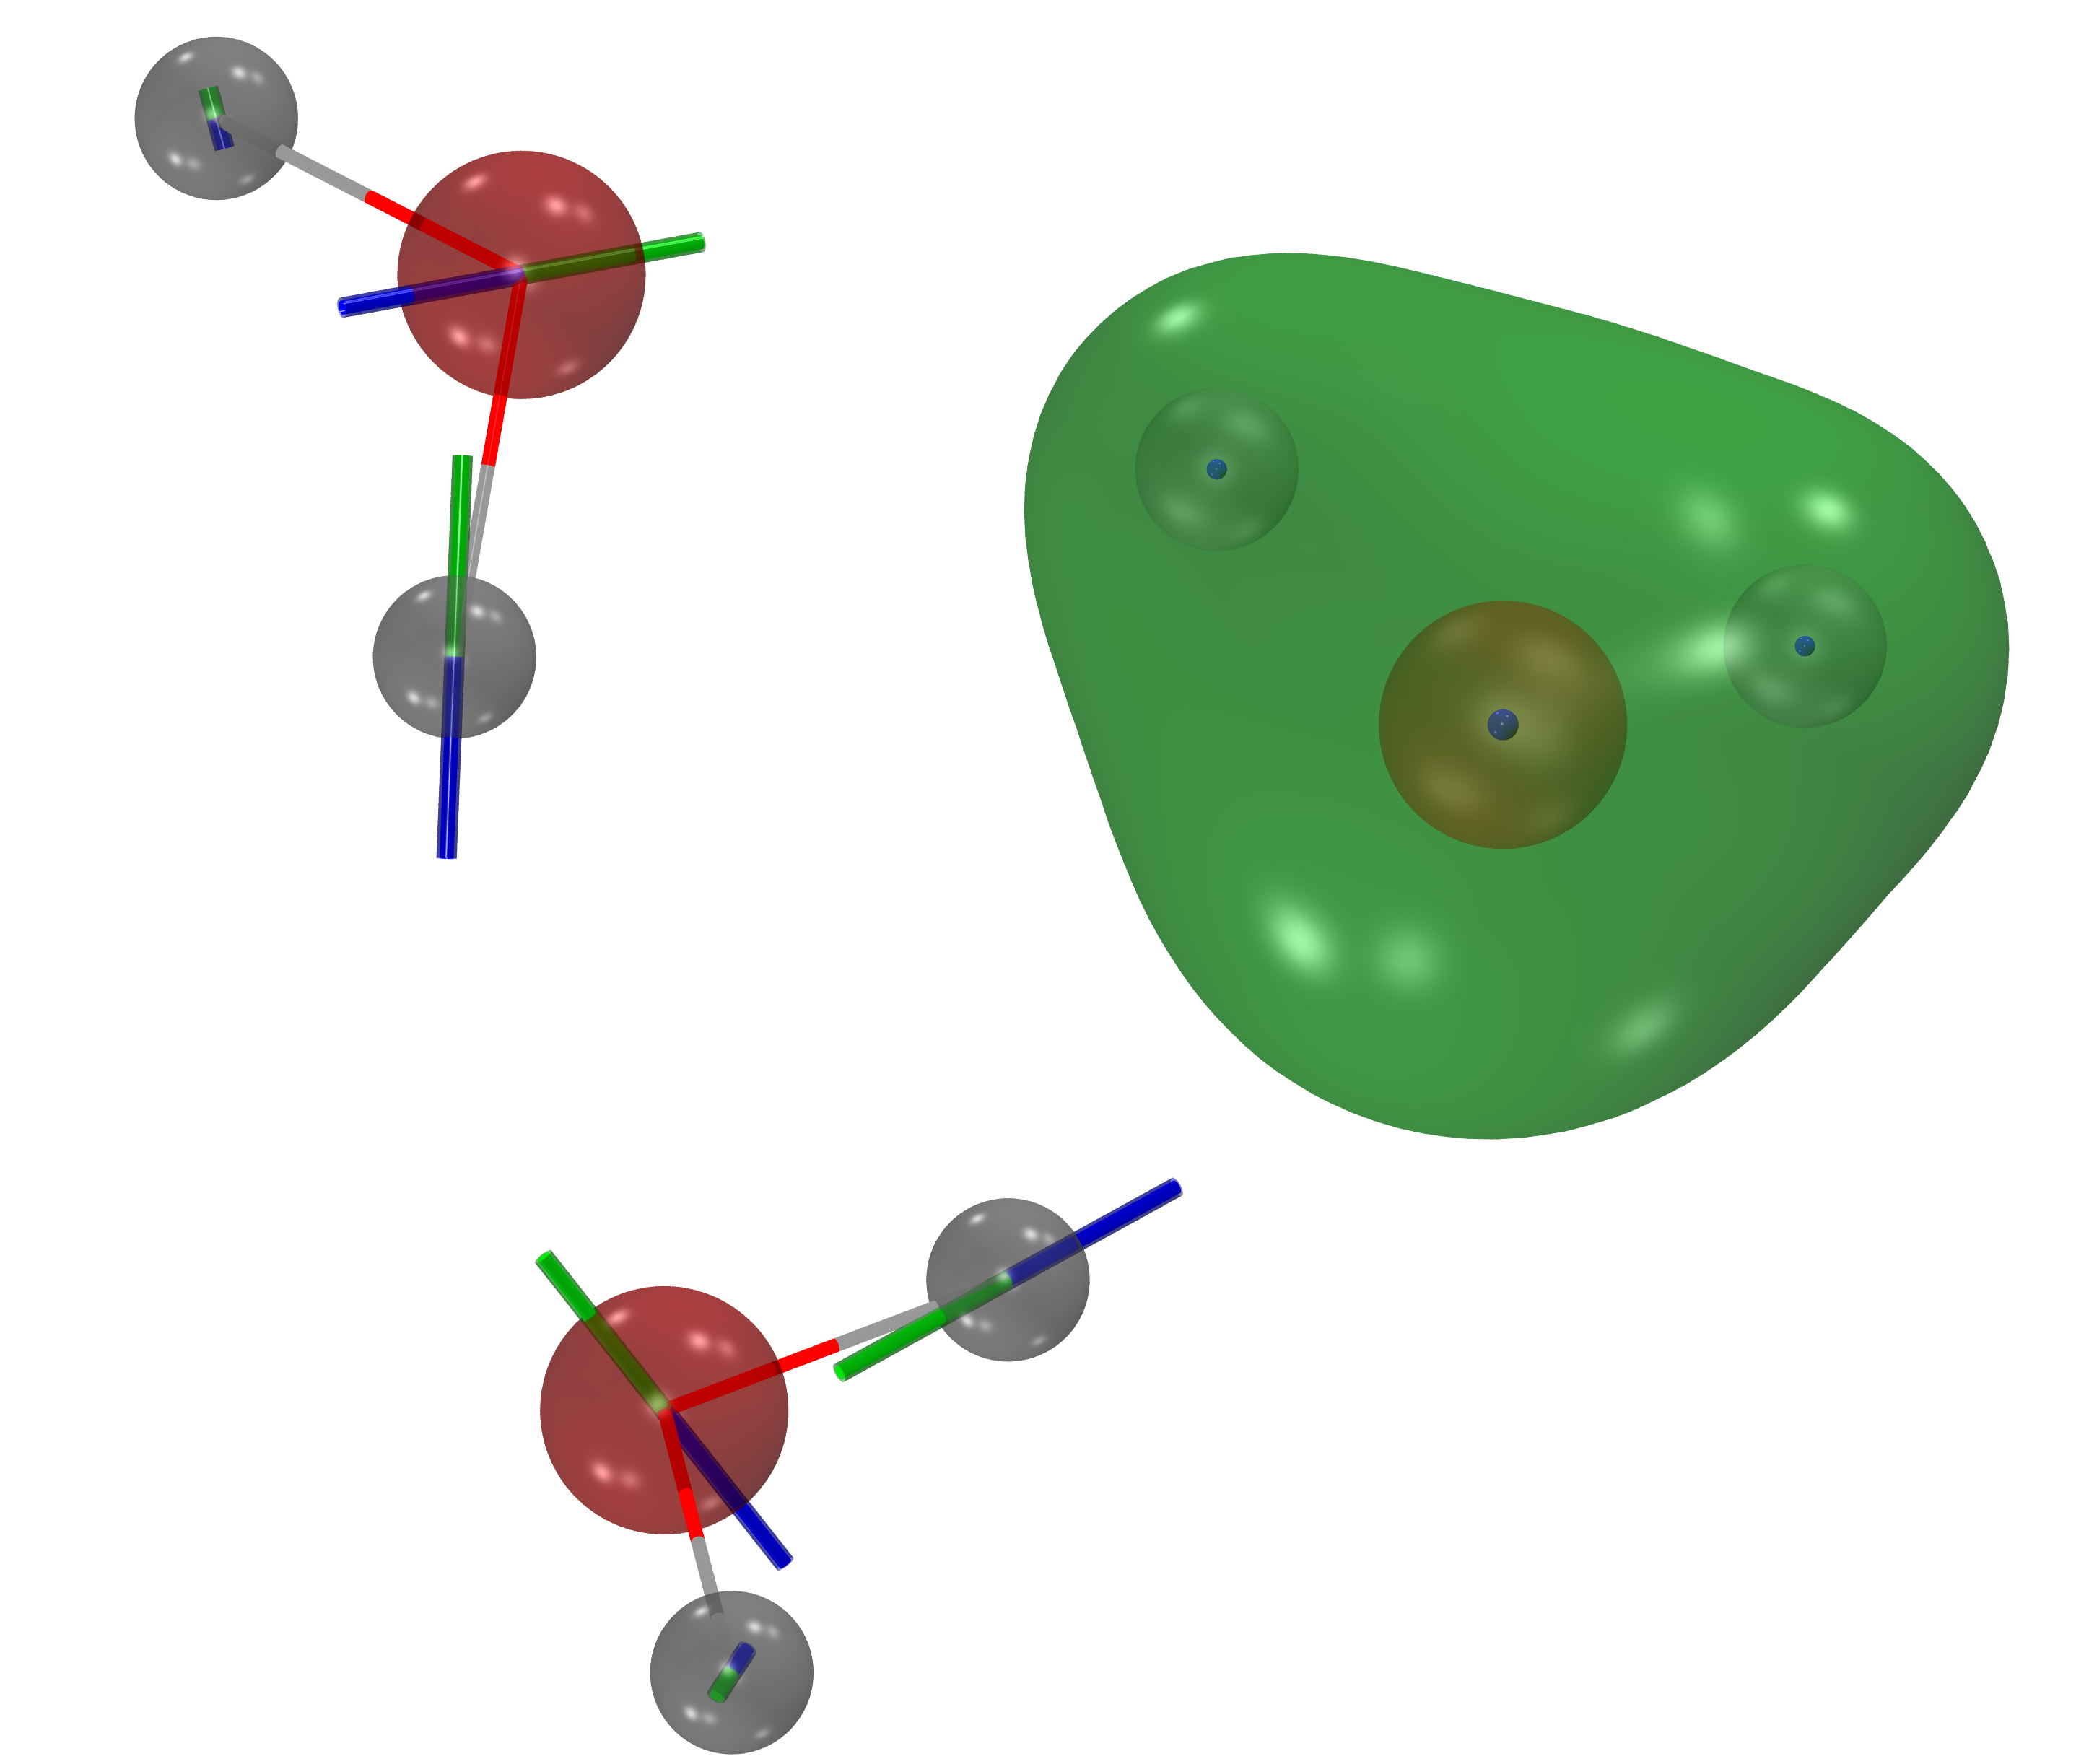
\includegraphics[scale=0.1]{../doc/images/trimer.png}
\end{center}}
\author{A QMMM Interface for Polarizable Force Fields}
\date{Eric G.\ Kratz, 2015}

%Main document
\begin{document}
\maketitle
\tableofcontents

\chapter{Introduction}

\section{Design Principles}

LICHEM is in development with four guiding principles: \\
\begin{quote}
 \normalfont{
 1) {\textbf{LICHEM should primarily be an interface.}}
 In order to make the code function with a variety of software packages and
 for different versions of the packages, LICHEM should not require
 modifications to other software packages or tools. \\
 2) {\textbf{LICHEM should be a single executable.}}
 Since LICHEM is an interface, there is no need for a large collection of
 binaries.
 Having many different single-use executable files can discourage new users.
 Furthermore, LICHEM can be statically linked to ease distribution of the
 software. \\
 3) {\textbf{LICHEM should be easy to read and modify.}}
 Most scientists  are not experts in computer programming.
 In order to allow for rapid collaborative development of LICHEM, the source
 code needs to be easy to read.
 To that end, the code should be simple, well commented, and avoid linking to
 esoteric libraries. \\
 4) {\textbf{LICHEM should be open source.}}
 LICHEM is licensed under the GPLv3.
 Science can benefit everyone, and hence, should be shared as widely as
 possible.
 Additionally, I do  not want to see my effort in creating a large software
 package go to waste in a package that can only be used by a handful
 of scientists.}
\end{quote}

\section{Notes for developers}

\subsection{Language and style}

The LICHEM repository contains code written in C++, \LaTeX, and markdown.
All lines of code should be less than 80 characters wide.
This has nothing to do with compiling or tracking changes, but helps to make
the code readable on smaller portable devices such as tablets and netbooks.
Also for readability purposes, avoid tabulars for indenting.
Tabulars can appear to be different sizes in some text editors. \\

When updating the documentation, there should be a newline after each
sentence.
This makes the documentation files very long, but it makes tracking/merging
changes safer and easier.
Paragraphs are ended with a \LaTeX\ newline followed by a blank line.

\subsection{Updating LICHEM}

Most of the development of LICHEM should be done though git (or other version
control packages) and merged into the main repository.
Since LICHEM does not require a large number of libraries or proprietary
software, it should be easy to share new wrappers and approximations with the
community.
Additionally, new wrappers and approximations should be placed into separate
files. \\

When functionality is added to LICHEM, the goal should be to make it simple
and robust.
Avoid adding lots of input keywords and extra input files.
It is better to have software that is a bit costly and always works than
software that is fast and tempermental.
A good example of this can be seen in the keywords used by the Gaussian
wrapper: \\

Int=UltraFine SCF=(YQC,Big,Direct) \\

Ultra-fine integrals and quadratic convergence (YQC) are certainly overkill
for most QM calculations, however, these options assure that difficult cases
will converge.
Additionally, the "Direct", YQC, and "Big" options are helpful for
larger systems, but they are not disabled for small systems.
Most of the wrappers contain assumptions that the QMMM calculations will be
large and quite difficult to simulate.
These sorts of options ensure that LICHEM will work on all systems without
requiring the user to be an expert with the QM and MM software. \\

LICHEM should be tested with extremely difficult systems.
During the early stages of the development, test systems with highly distorted
structures were employed to make sure that crashing the software was rare.

A simple way to avoid modifying the QM and MM packages is to search for
iterative or perturbative approximations for the QMMM equations.
This is extremely useful for multipolar/polarizable force fields.

\subsection{Parallelization}

LICHEM is parallelized with OpenMP, however, the packages called by the
wrappers can use any form of parallelization.
Care must be taken to avoid creating too many threads when calling multiple
parallel functions with the wrappers. \\

In multi-replica simulations, the number of CPUs given as a command line
argument is used to divide the OpenMP threads between the replicas.
As more MPI enabled packages are included in the wrappers, the parallelization
paradigm will be adjusted.
The current OpenMP thread settings can be found in the ReadLICHEMInput()
routine.

\section{Installation}

Since LICHEM is designed to be simple, only a small number of packages are
required to compile the code.
An approximate list of packages is given below.
\begin{quote}
 \normalfont{
 LICHEM binary: OpenMP, Eigen3 \\
 LICHEM manual: LaTeX, BibTex, TeXLive}
\end{quote}

To install LICHEM, clone the git repository \\

user:\$ mkdir LICHEM \\
user:\$ git clone https://github.com/kratman/LICHEM\_QMMM.git ./LICHEM/ \\

or unpack the zipped source code \\

user:\$ mkdir LICHEM \\
user:\$ cd LICHEM/ \\
user:\$ unzip LICHEM\_QMMM-master.zip \\
user:\$ mv LICHEM\_QMMM-master/* . \\
user:\$ rmdir LICHEM\_QMMM-master \\

The LICHEM binary will eventually be included with the zipped source code,
however, modified or git source code can be compiled with the Makefile
provided with LICHEM.
On Ubuntu boxes, the Makefile should function without modifications.
However, with other operating systems it may be necessary to change the path
to the \textit{Eigen3} package. \\

Default: -I/usr/include/eigen3/ \\

The Makefile can produce both the documentation and the binary. \\

user:\$ make install \\

Although, if you are reading this then you already have the documentation. \\

For development, debugging, or testing an alternate binary can be compiled. \\

user:\$ make Dev \\

Additional make rules can be found in the Makefile.

\section{Capabilities}

\begin{table}[hbt]
 \centering
 \begin{tabular}{|c|c c c|}
 \hline
  & Gaussian & PSI4 & NWChem \\ \hline
 QM energy & Yes & Yes & Yes \\
 QMMM energy & Yes & Yes & Yes \\ \hline
 QM opt. & Yes & Yes & No \\
 QMMM opt. & Yes & No & No \\ \hline
 QM SD/DFP & Yes & Yes & Yes \\
 QMMM SD/DFP & Yes & No & Yes \\ \hline
 QM MC & Yes & Yes & Yes \\
 QMMM MC & Yes & Yes & Yes\\ \hline
 QM PIMC & Yes & Yes & Yes \\
 QMMM PIMC & Yes & Yes & Yes \\ \hline
 QM RP & Yes & No & Yes\\
 QMMM RP & Yes & No & Yes \\ \hline
 \end{tabular}
 \caption{
 QM wrapper capabilities for single-point energy, geometry optimization,
 steepest descent or Davidon-Fletcher-Powell (SD/DFP), Monte Carlo (MC),
 path-integral Monte Carlo (PIMC), and reaction path (RP) calculations.}
 \label{tab:QMWrapCap}
\end{table}

\begin{table}[hbt]
 \centering
 \begin{tabular}{|c|c c c|}
 \hline
  & TINKER & AMBER & LAMMPS \\ \hline
 MM energy &  Yes & Yes & Yes \\
 QMMM energy & Yes & Yes & Yes \\ \hline
 MM opt. & Yes & Yes & Yes \\
 QMMM opt. & Yes & Yes & Yes \\ \hline
 MM SD/DFP & No & No & No \\
 QMMM SD/DFP & Yes & Yes & Yes \\ \hline
 MM MC & Yes & Yes & Yes \\
 QMMM MC & Yes & Yes & Yes \\ \hline
 MM PIMC & Yes & Yes & Yes \\
 QMMM PIMC & Yes & Yes & Yes \\ \hline
 MM RP & No & No & No \\
 QMMM RP & Yes & Yes & Yes \\ \hline
 \end{tabular}
 \caption{
 MM wrapper capabilities for single-point energy, geometry optimization,
 steepest descent or Davidon-Fletcher-Powell (SD/DFP), Monte Carlo (MC),
 path-integral Monte Carlo (PIMC), and reaction path (RP) calculations.}
 \label{tab:MMWrapCap}
\end{table}

\subsection{QM and MM wrappers}

LICHEM can perform QM, MM, or QMMM calculations via an interface to packages
in the user's path.
Temporary input files are created for each package and the results are
collected from the temporary output files.
This is a relatively inefficient procedure, however, reading and writing
input/output files is often negligible compared to the computational cost of
the QM calculation.
Currently, calculations can be performed using Gaussian \cite{Frisch2009},
PSI4 \cite{Turney2012}, TINKER \cite{Ponder2015}, AMBER \cite{Case2015}, and
LAMMPS \cite{Plimpton1995}.
Additional wrappers can be added to LICHEM with relatively little effort.

\subsection{Types of calculations}

Single-point energies, geometry optimizations, steepest descent minimizations,
reaction pathways, ensemble sampling, classical Monte Carlo, and
path-integral Monte Carlo calculations can be performed using the QM and MM
wrappers.
Due to limitations of the software packages, not all calculations can
currently be performed with all combinations of wrappers.
For convenience, the capabilities are summarized in Table \ref{tab:QMWrapCap}
and \ref{tab:MMWrapCap}. \\

Some additional restrictions are also present when there are bonds between
the QM and MM regions.
Currently PSI4 cannot be used as a QM wrapper for calculations where the QM
and MM regions are bonded.

\section{Acknowledgements}

The development of LICHEM was supported by funding from the NIH (Grant No.\
R01GM108583) and Wayne State University.
LICHEM is maintained by the Cisneros research group at Wayne State University.

\chapter{LICHEM Input}

\section{Command line arguments}

LICHEM can only be invoked from a command line interface. \\

user:\$ lichem -n Ncpus -x xyzfile.xyz -c confile.inp
-r regfile.inp -o output.xyz \\

-n: Number of CPUs used in the calculations.
Note that during PIMC and reaction path calculations each replica uses this
many CPUs.
A reaction path calculation with 8 points and Ncpus=2 may require 16 CPUs. \\

-x: File name for the input structure in XYZ format.
The XYZ input should be in the standard format and have a blank comment
line. \\

-c: File name for connectivity and force field information. \\

-r: File name for definitions of QMMM regions, QM wrapper, MM wrapper,
and general simulation options. \\

-o: File name for trajectories and optimized structures.

\section{XYZ input files}

The input structure for LICHEM is a standard XYZ file with a blank comment
line. \\

N \\

A  X$_A$  Y$_A$  Z$_A$ \\
B  X$_B$  Y$_B$  Z$_B$ \\
... \\

Here N is the number of atoms and (X$_i$,Y$_i$,Z$_i$) is the position of
particle $i$.
Note that the atom types given in the XYZ file need to be the atomic symbols
from the periodic table, not the MM atom types.
Additionally, LICHEM reads the XYZ file item-by-item, which means that having
additional values on a line will cause (silent) errors.

\section{Connectivity input files}

The connectivity of the molecules and the force field information are defined
in the connectivity file.
The general format is given below. \\

id MMTyp NumTyp q Nbonds [connectivity] \\
... \\

Here id is the index of the atom (0 to N-1), MMTyp is the force field atom
type (i.e.\ AMBER atom types), NumTyp is a numerical atom type (i.e.\ TINKER
atom types), q is the force field charge on the atom, Nbonds is the number of
bonds to the atom, and [connectivity] is the bond list.
The length of the connectivity list must match Nbonds and the information in
the connectivity file must be given for all atoms, even if there are no MM
atoms in the system.
During pure QM simulations, most of the connectivity information is ignored.
An additional caveat is that the atoms must be listed in order.
This is part of an internal check to make sure correct input files were
provided.

\section{Region input files}

The region file contains QMMM regions (QM atoms, pseudo-bond atoms, boundary
atoms, and frozen atoms) as well as miscellaneous input needed to define the
type of calculations that will be performed.
This is the most complicated input file required by LICHEM and currently the
input keywords must be given in the correct order.
The keywords themselves are only guides for making the files human readable
and only the values after the keywords are read.
Blank templates of region files are provided in the documentation
directory. \\

The first line of the input file should read: \\

Potential\_type: $<$QM or MM or QMMM$>$ \\

This line tells LICHEM what type of QM and MM input is listed in the lines
that follow.

\subsection{General notes}

Input that is not specific to the wrappers is mostly case insensitive,
however, users may find exceptions to this rule of thumb.
Future versions of LICHEM will have a more robust input reader.
In the mean-time, please report any bugs that are found.
Some input errors will be caught by the error checking functions.

\subsection{QM input}

If the potential type is QM or QMMMM, several keywords are required to define
the QM wrapper and level of theory. \\

QM\_type: $<$Gaussian or PSI4 or NWChem$>$ \\
QM\_method: $<$HF or functional or SemiEmp$>$ \\
QM\_basis: $<$basis set or model$>$ \\
QM\_memory: $<$RAM$>$ $<$MB or GB$>$ \\
QM\_charge: $<$charge on the QM region$>$ \\
QM\_spin: $<$multiplicity of the QM region$>$ \\

All of the QM input is read into LICHEM as text, and hence, it must match the
correct input for the QM package.
For example, Gaussian can only read integer values for the memory.
If the QM method is set to SemiEmp, then the QM basis should be set to the
semi-empirical model Hamiltonian.

\subsection{MM input}

If the potential type is MM or QMMM, several keywords are required to define
the MM wrapper. \\

MM\_type: $<$TINKER or AMBER or LAMMPS$>$ \\
Electrostatics: $<$Charges or AMOEBA or Density$>$ \\

\subsection{QMMM input}

QMMM input is a combination of the QM and MM input described above. \\

QM\_type: $<$Gaussian or PSI4 or NWChem$>$ \\
QM\_method: $<$HF or functional or SemiEmp$>$ \\
QM\_basis: $<$basis set or model$>$ \\
QM\_memory: $<$RAM$>$ $<$MB or GB$>$ \\
QM\_charge: $<$charge on the QM region$>$ \\
QM\_spin: $<$multiplicity of the QM region$>$ \\
MM\_type: $<$TINKER or AMBER or LAMMPS$>$ \\
Electrostatics: $<$Charges or AMOEBA or Density$>$ \\

All of the QMMM input is read into LICHEM as text, and hence, it must match the
correct input for the QM and MM packages.
For example, Gaussian can only read integer values for the memory.
If the QM method is set to SemiEmp, then the QM basis should be set to the
semi-empirical model Hamiltonian.

\subsection{Simulation input}

Input for the calculation types directly follows the wrapper input.
Each type of calculation requires slightly different input.
LICHEM can perform single-point energies (SP), geometry optimizations
(Opt,DFP,ESD,Steep,NEB), and path-integral Monte Carlo simulations (PIMC).
Classical Monte Carlo simulations can be performed as PIMC simulations with a
single bead. \\

A description of the methods are given in Chapter \ref{chap:Theory} and the
input for all calculation types are documented below.
Synonyms for the simulation keywords are given in parentheses. \\

\subsubsection{Energy calculations}

Calculation\_type: Energy (or SP) \\

\subsubsection{Geometry optimizations}

There are currently three options for geometry optimizations in LICHEM.
The optimization types only differ in the method used to optimize the
QM atoms.
MM atoms are always optimized using the native MM wrappers. \\

Calculation\_type: Opt \\
Max\_opt\_step: $<$Size of the maximum optimization step (\AA)$>$ \\
MM\_opt\_tolerance: $<$Criteria to stop MM optimization$>$ \\
Max\_opt\_steps: $<$Run at most N QM steps per iteration$>$ \\

The Opt keyword performs a geometry optimization using the native optimization
routines in the QM package.
Pure QM systems can be optimized with any of the QM packages, but only
Gaussian can be used for QMMM optimizations with this keyword. \\

Calculation\_type: Steep (or SD) \\
Opt\_step\_size: $<$Initial scale factor for the step size$>$ \\
Max\_opt\_step: $<$Size of the maximum optimization step (\AA)$>$ \\
QM\_opt\_tolerance: $<$Criteria to stop the QM optimization$>$ \\
MM\_opt\_tolerance: $<$Criteria to stop MM optimization$>$ \\
Max\_opt\_steps: $<$Run at most N QM steps per iteration$>$ \\

LICHEM has a steepest descent routine which optimizes the structure in
Cartesian coordinates. \\

Calculation\_type: QuickMin (Quick or DV) \\
Opt\_step\_size: $<$Time step (arbitrary units)$>$ \\
Max\_opt\_step: $<$Size of the maximum optimization step (\AA)$>$ \\
QM\_opt\_tolerance: $<$Criteria to stop the QM optimization$>$ \\
MM\_opt\_tolerance: $<$Criteria to stop MM optimization$>$ \\
Max\_opt\_steps: $<$Run at most N QM steps per iteration$>$ \\

LICHEM has a damped Verlet routine which optimizes the structure in
Cartesian coordinates. \\

Calculation\_type: DFP \\
Opt\_step\_size: $<$Initial scale factor for the step size$>$ \\
Max\_opt\_step: $<$Size of the maximum optimization step (\AA)$>$ \\
QM\_opt\_tolerance: $<$Criteria to stop the QM optimization$>$ \\
MM\_opt\_tolerance: $<$Criteria to stop MM optimization$>$ \\
Max\_opt\_steps: $<$Run at most N QM steps per iteration$>$ \\

LICHEM has a built in Davidon-Fletcher-Powell (DFP) optimizer.
Like the steepest descent routine, the DFP optimizer uses Cartesian
coordinates.

\subsubsection{Reaction path optimizations}

LICHEM has built in reaction path and transition state optimizers. \\

Calculation\_type: NEB \\
Number\_of\_beads: $<$Number of replicas, must be odd$>$ \\
Opt\_step\_size: $<$Initial scale factor for the step size$>$ \\
Max\_opt\_step: $<$Size of the maximum optimization step (\AA)$>$ \\
Spring\_constant: $<$NEB spring constant (eV/\AA$^2$)$>$ \\
Frozen\_ends: $<$Yes or No$>$ \\
QM\_opt\_tolerance: $<$Criteria to stop the QM optimization$>$ \\
MM\_opt\_tolerance: $<$Criteria to stop MM optimization$>$ \\
Max\_opt\_steps: $<$Run at most N QM steps per iteration$>$ \\

The NEB method implemented in LICHEM is the climbing
image nudged elastic band method.
The replica with the highest energy moves upwards along the reaction
path to locate a transition state.
For more details on the method, see Chapter \ref{chap:Theory}.

\subsubsection{Ensemble samping and Monte Carlo}

Calculation\_type: EnsembleSD (or ESD) \\
Opt\_step\_size: $<$Scale factor for the step size$>$ \\
Max\_opt\_step: $<$Maximum displacement for each step (\AA)$>$ \\
QM\_opt\_steps: $<$Perform N QM steps$>$ \\
Timestep: $<$MD timestep (fs)$>$ \\
Temperature: $<$MD temperature (K)$>$ \\
Tau: $<$Thermostat time constant ($\tau$)$>$ \\
MD\_steps: $<$Run N MD steps per QM step$>$ \\

Calculation\_type: EnsembleNEB (or ENEB) \\
Number\_of\_beads: $<$Number of replicas, must be odd$>$ \\
Opt\_step\_size: $<$Scale factor for the step size$>$ \\
Max\_opt\_step: $<$Maximum displacement for each step (\AA)$>$ \\
Spring\_constant: $<$NEB spring constant (eV/\AA$^2$)$>$ \\
QM\_opt\_steps: $<$Perform N QM steps$>$ \\
Timestep: $<$MD timestep (fs)$>$ \\
Temperature: $<$MD temperature (K)$>$ \\
Tau: $<$Thermostat time constant ($\tau$)$>$ \\
MD\_steps: $<$Run N MD steps per QM step$>$ \\

Calculation\_type: PIMC \\
Ensemble: $<$NVT or NPT$>$ \\
Temperature: $<$Temperature in Kelvin$>$ \\
Pressure: $<$Pressure in atm $>$ \\
Number\_of\_eq\_steps: $<$Run N steps before collecting data$>$ \\
Number\_of\_MC\_steps: $<$Collect data for N steps$>$ \\
Number\_of\_beads: $<$Number of PI beads$>$ \\
Acceptance\_ratio: $<$Fraction of attempted moves which succeed$>$ \\
Traj\_steps\_before\_printing: $<$Print every N steps$>$ \\

\subsection{Region input}

Four different regions of the structure need to be defined even if the
regions contain zero atoms. \\

QM\_atoms: Nqm [list of ids] \\
Pseudobond\_atoms: Npseudo [list of ids] \\
Boundary\_atoms: Nbound [list of ids] \\
Frozen\_atoms: Ninact [list of ids] \\

Definitions of the QM, pseudo-bond atoms, and boundary atoms can be found in
Chapter \ref{chap:Theory}.
Frozen atoms are MM atoms that should remain stationary during optimizations,
dynamics, or Monte Carlo simulations.
Frozen atoms are useful for optimizing small regions of large periodic
systems. \\

Note that in pure QM and pure MM simulations, \{Nqm,Npseudo,Nbound\} can all
be set to zero.
This is because these regions are not relevant unless LICHEM is performing a
QMMM calculation.
For all of the regions, the lists of atoms can be separated by either spaces
or newlines.

\section{File conversion}

While LICHEM does not handle atom typing or structure generation, it is
possible to use the native input/output functions to create LICHEM input from
input used for QM and MM packages.
In all cases the converter produces three files: xyzfile.xyz connect.inp
regions.inp \\

{\textbf{Gaussian/NWChem}} \\

LICHEM can use a region file to create a BASIS set file for the Gaussian
and NWChem basis set input.
A BASIS file is required when mixed basis sets or pseudobonds are included
in the QMMM calculations. \\

user:\$ lichem -convert -b regions.inp \\

The convert flag checks for specific keywords in the region file to construct
a BASIS file in the correct order. \\

Required keywords: \\
'QM\_type:' \\
'QM\_basis:' \\
'QM\_atoms:' \\
'Pseudobond\_atoms:' \\

Currently, these keywords must be spelled and formatted exactly as given
above. \\

{\textbf{TINKER:}} \\

The file converter for TINKER can be used on standard TINKER XYZ files,
TINKER QMMM XYZ files (g09MM2,Q-CHEM), and TINKER XYZ files with periodic
boundary conditions. \\

user:\$ lichem -convert -t TINKER.xyz -k tinker.key ( -p Yes) \\

The -p flag is optional and tells LICHEM to read the lattice constants from
the second line of the XYZ file. \\

LICHEM can also be used to create TINKER xyz files: \\

user:\$ lichem -tinker -x xyzfile.xyz -c connectfile.inp \\

A file called "tinkxyz.xyz" will be produced from this conversion. \\

The GlobalPoles flag reads the force field and initial structure, then prints
the multipoles in the global reference frame. \\

user:\$ lichem -GlobalPoles -n Ncpus -x xyzfile.xyz -r regions.inp
 -c connect.inp \\

{\textbf{AMBER:}} \\

{\color{red}Still in development} \\

{\textbf{LAMMPS:}} \\

{\color{red}Still in development}

\section{LICHEM output}

Most of the LICHEM output is sent through the c++ std output stream.
However, trajectories and optimized structures are printed into the file
defined by the -o flag.
In single-point energy calculations, the output XYZ file is deleted after the
calculation is completed, since the geometry does not change during the
calculation.
LICHEM also leaves some restart files in theworking directory (e.g.\ Gaussian
checkpoint files, multi-replica XYZ files, etc).

\section{Additional input for wrappers}

The LICHEM wrappers automatically look for a couple "extra" input files.
These files depend on which wrappers are used in the calculation, however, in
most cases the files contain force field and pseudopotential information.
Some of the extra files are detailed below in no particular order and examples
can be found in the documentation directory.

\subsection{TINKER}

The TINKER wrapper checks the working directory for a file called tinker.key
and will read additional force field information (e.g.\ atom classes,
multipoles, etc) based on the keywords listed in that file.
Any keyword defined in tinker.key will be passed into the TINKER key file used
by the wrapper.
For obvious reasons, the user must also provide the force field parameter
files defined in the tinker.key file.

\subsection{AMBER}

{\color{red}Still in development}

\subsection{LAMMPS}

{\color{red}Still in development}

\subsection{Gaussian}

The Gaussian wrapper will look for checkpoint files and a file called BASIS in
the working directory.
The BASIS file contains basis set and pseudopotential information for QMMM
calculations with bonds between the QM and MM regions (see below).
While the file is read in automatically if it is found, the user still needs
to tell Gaussian to use this information: \\

QM\_basis: GEN \\

GEN is a Gaussian keyword which causes the package to check for extra basis
set information below the structure. \\

LICHEM automatically tells Gaussian to look for pseudopotentials, however,
these must be given below the basis set information in the BASIS file.
Both the basis set and pseudopotential information must be given in Gaussian
format.

\subsection{NWChem}

The NWChem wrapper will look for checkpoint files and a file called BASIS in
the working directory.
The BASIS file contains basis set and pseudopotential information for QMMM
calculations with bonds between the QM and MM regions (see below).
If the BASIS file is found, then the basis set given in the regions file is
ignored.
Both the basis set and pseudopotential information must be given in NWChem
format.

\subsection{Restart files}

While restarting incomplete geometry optimizations only requires changing
the initial structure given with the -x flag, multi-replica simulations
require structural information for each replica.
When a multi-replica (PIMC or reaction path) simulation is started LICHEM
checks the working directory for a restart file named "BeadStartStruct.xyz"
which will be used as the initial structure.
The restart file is similar to a standard XYZ file, except all the replicas
are merged together (see below). \\

M \\

A  X$_{A,0}$  Y$_{A,0}$  Z$_{A,0}$ \\
A  X$_{A,1}$  Y$_{A,1}$  Z$_{A,1}$ \\
... \\
A  X$_{A,M-1}$  Y$_{A,M-1}$  Z$_{A,M-1}$ \\
B  X$_{B,0}$  Y$_{B,0}$  Z$_{B,0}$ \\
B  X$_{B,1}$  Y$_{B,1}$  Z$_{B,1}$ \\
... \\

Here M is the number of atoms times the number of beads, and
(X$_{i.j}$,Y$_{i,j}$,Z$_{i,j}$) is the position of particle $i$ in replica
$j$.
Note that the atom types given in the XYZ file are ignored since this
information is read from the files given by the -x and -c flags.

\subsection{Examples and tests}

Example LICHEM input and tutorials can be found in the doc directory.
Most of the examples are not intended to be used for calculations. \\

Gaussian\_files: Example files for Gaussian basis and pseudopotential
input (e.g. BASIS). \\

PDB\_input: A tutorial for creating LICHEM (Gaussian/TINKER) input from a
PDB file.
The PDB tutorial contains complete input to run a single-point energy
calculation on a peptide chain. \\

Region\_files: Example region files for a variety of calculations. \\

TINKER\_files: Contains tinker.key files. \\

LICHEM also has a semi-automated test suite. \\

user:\$ ./runtests [Ncpus] [QM package] [MM package] [dry (optional)] \\

The test suite searches for QM and MM binaries matching the given names
and runs a set of single-point energy calculations.
If no arguments are given to runtests, the test suite will print all available
QM and MM binaries.
A dry run can also be performed, where the test suite does not run any of the
actual calculations.

\chapter{Theoretical Background}
\label{chap:Theory}

\section{Preface}

The following chapter is intended to serve as a general introduction to
computational chemistry and the methods used in LICHEM.
There are numerous places users can find more detailed and up-to-date
discussions of these topics.
This chapter is only intended to give a broad review of the concepts and
terminology.

\section{Classical Methods}

\subsection{Newton's laws of motion}

Much of classical physics can be described in terms of Newton's three laws of
motion.
\begin{quote}
 \normalfont{
 1) An object in motion tends to stay in motion unless it is acted upon by a
 force. \\
 2) The force on an object is equal to its mass times its acceleration
 ($F=ma$). \\
 3) For every action, there is an equal and opposite reaction.}
\end{quote}
Newton's second law can be employed in calculations to predict the position
and velocity of objects moving in a potential field.
A simplified algorithm for the discretized equations of motion can be written
as
\begin{equation}
 F_{n} = -\nabla V_{n} = m\ddot {\textbf r}_{n} \; ,
\end{equation}
\begin{equation}
 \dot {\textbf r}_{n+1} = \dot {\textbf r}_{n}+\ddot {\textbf r}_{n}
 \Delta t \; ,
\end{equation}
and
\begin{equation}
 {\textbf r}_{n+1} = {\textbf r}_{n}+\dot {\textbf r}_{n}\Delta t
 +\frac{\ddot {\textbf r}_{n}\Delta t^2}{2} \; ,
\end{equation}
where $F$ is the force, $V$ is the potential energy, $\textbf{r}$ is a vector
representing the positions of all atoms in the system, and $\Delta t$ is the
time interval between step $n$ and $n+1$.
The natural ensemble for molecular dynamics is the microcanonical ensemble
(NVE), where the number of particles and energy are conserved inside a
constant volume simulation box.
Although the NVE simulations are the native result of propagating Newton's
equations, most experiments are performed in the canonical (NVT) or
isothermal-isobaric (NPT) ensembles.
In the NVT ensemble, the temperature is held constant instead of the energy,
and the NPT ensemble also holds the pressure to be constant by adjusting the
size of the simulation box.

\subsection{Force fields}

Empirical force fields are classical potentials which can estimate the
potential energy of a system.
Although any functional form could be employed for the force field, the
potentials are often derived from experiments, classical physics, or quantum
theory. \\

Non-bonded interactions of atoms are typically modeled using point-charges
and Lennard-Jones potentials or other van der Waals potentials.
The non-bonded potential is given by
\begin{equation}
 V(R) = V_{coul}(R)+V_{vdW}(R) \; ,
\end{equation}
\begin{equation}
 V_{coul}(R) = C\sum \frac{q_iq_j}{r_{ij}} \; ,
\end{equation}
and
\begin{equation}
 V_{vdW}(R) = \sum \frac{A_{ij}}{r_{ij}^{12}}
              -\frac{B_{ij}}{r_{ij}^{6}} \; ,
\end{equation}
where $R$ is a vector representing the coordinates of the system, $V(R)$ is the
potential, $V_{coul}(R)$ is the Coulomb potential for point-charges ($q$),
$C$ is a constant, $r_{ij}$ is the distance between atoms $i$ and $j$,
$V_{vdW}(R)$ is the van der Waals potential (in this case, the Lennard-Jones
potential), $A_{ij}$ is a parameter representing the exchange interaction, and
$B_{ij}$ is a parameter representing the dispersion interaction. \\

Bonded interactions are often represented by the harmonic potential.
Harmonic bonds behave as idealized springs that never weaken or break.
The harmonic potential is given by
\begin{equation}
 V_{harm}(r_{ij}) = \frac{K_{ij}}{2}r_{ij}^2 \; ,
\end{equation}
where $K_{ij}$ is the spring constant.
Similarly, bond angles can be described by a harmonic potential
\begin{equation}
 V_{harm}(\theta_{ijk}) = \frac{K_{ijk}}{2}\theta_{ijk}^2 \; ,
\end{equation}
where $\theta$ is the angle between atoms $i$, $j$, and $k$.
More complicated potentials can be constructed for the bonded interactions,
but these are two of the most common potentials.
Typically, large molecules require potentials for dihedral angles and improper
dihedral angles. \\

The parameters for force fields are determined in a very systematic fashion.
Typically, the charges are determined from electronic structure calculations
and bonded parameters are determined by matching the molecular vibrational
modes.
The van der Waals parameters are usually adjusted to reproduce the density,
enthalpy of freezing, or other experimentally determined properties.

\subsection{Polarizable force fields}

Point-charges are often inadequate for representing the electrostatic field
around a molecule.
The field can be improved by assigning point-charges ($q$), dipoles ($\mu$),
quadrupoles ($\Theta$), and polarizabilities ($\alpha$) to the atoms.
These force fields are more computationally expensive than standard
point-charge force fields, however, the results can be much more accurate. \\

Multipoles add an additional complication to the potential in that the
potential is aspherical.
To address this, a local frame of reference is defined for each atom.
Local frames are defined using two or three neighboring atoms. \\

A Cartesian representation of the multipoles can be simplified by converting
to a spherical harmonic representation.
The first step in the conversion is to diagonalize the quadrupole tensor
\begin{equation}
 R^{-1}\Theta R = \Theta' \; ,
\end{equation}
where $R$ are the eigenvectors and $\Theta'$ are the eigenvalues.
The Cartesian multipoles through the quadrupole moments can be converted to
the spherical harmonic multipoles, $Q$
\begin{equation}
 Q_{00} = q \; ,
\end{equation}
\begin{equation}
 Q_{11c} = \vec \mu \cdot R_x \; ,
\end{equation}
\begin{equation}
 Q_{11s} = \vec \mu \cdot R_y \; ,
\end{equation}
\begin{equation}
 Q_{10} = \vec \mu \cdot R_z \; ,
\end{equation}
\begin{equation}
 Q_{22c} = (\Theta_{xx}-\Theta_{yy})/\sqrt{3} \; ,
\end{equation}
\begin{equation}
 Q_{20} = \Theta_{zz} \; ,
\end{equation}
where $R_i$ are the eigenvectors in the $i$ direction.
The spherical harmonic representation reduces the the multipole expansion to
six moments in the new frame of reference defined by $R$. \cite{} \\

The spherical harmonic multipole expansion through quadrupole moments can be
converted to six point-charges. \cite{}
\begin{equation}
 q_{\pm x} = \frac{Q_{00}}{6} \pm \frac{Q_{11c}}{2d} -
          \frac{Q_{20}}{6d^2} + \frac{Q_{22c}}{2\sqrt{3}d^2} \; ,
\end{equation}
\begin{equation}
 q_{\pm y} = \frac{Q_{00}}{6} \pm \frac{Q_{11s}}{2d} -
          \frac{Q_{20}}{6d^2} - \frac{Q_{22c}}{2\sqrt{3}d^2} \; ,
\end{equation}
\begin{equation}
 q_{\pm z} = \frac{Q_{00}}{6} \pm \frac{Q_{10}}{2d} +
          \frac{Q_{20}}{3d^2} \; ,
\end{equation}
where $q_{\pm i}$ are the charges in the $\pm R_i$ direction, and $d$ is the
displacement from the atomic center.
Before the electrostatic interactions can be calculated, the point-charges
must be rotated from the local frame of reference to the global frame.
While representing the multipoles as a set of point-charges reduces the
accuracy, most QM and MM packages can easily add additional point-charges to
the potential.

\subsection{Polarizable density force fields}

Polarizable density force fields are a special class of polarizable force
fields where the electron density is represented by Gaussian functions.
These potentials can greatly improve the calculations of the electrostatic
field and can include exchange and charge penetration effects.

\section{Geometry and Reaction Path Optimizations}

\subsection{Steepest descent}

Steepest descent (SD) is the simplest optimization method.
The gradient of the potential is calculated at the current geometry and used
to update the atomic coordinates.
\begin{equation}
 {\textbf r}_{n+1} = {\textbf r}_n+\alpha_n \nabla V({\textbf r}) \; ,
\end{equation}
Here $V({\textbf r})$ is the potential at the set of coordinates
${\textbf r}$ and $\alpha$ is a scale factor which determines how far a
particle moves during step $n$. \\

Efficient SD optimizers use line search algorithms which backtrack to find the
optimum value of $\alpha$ at step $n$.
However, SD optimizations often do not converge even with optimal step
sizes. \\

The SD algorithm in LICHEM does not use a line search to optimize $\alpha$ at
each step.
Instead, a maximum value of $\alpha$ is given in the input and the
optimization starts with $\alpha=0.7\alpha_{max}$.
If the QMMM energy is decreasing, then the step size increases by 5\% until it
reaches $\alpha_{max}$.
If the energy increases, the step size is reduced by 40\% and the optimization
continues.

\subsection{Davidon-Fletcher-Powell}

SD optimizations move along the first derivative of the potential (gradient).
Optimzations are more efficient if the atoms move along a path chosen using
both the first and second derivatives of the potential.
The second derivative matrix (Hessian) can be expensive to calculate, however,
there are several quasi-Newton algorithms which can improve a guess Hessian.
The most common procedures are the Davidon-Fletcher-Powell (DFP) and
Broyden-Fletcher-Goldfarb-Shanno (BFGS) algorithms.
These two methods are mathematically related and can theoretically start from
any initial guess of the inverse Hessian, $H^{-1}$. \\

The DFP algorithm can update the inverse Hessian using the forces ($F_n$), the
current inverse Hessian, and the optimization vector ($p_n$).
The optimization algorithm is given by
\begin{equation}
 p_n = \alpha_n H_n^{-1} F_n \; ,
\end{equation}
\begin{equation}
 \delta_n = F_{n-1}-F_n \; ,
\end{equation}
and
\begin{equation}
 \label{eq:DFP}
 H_{n+1}^{-1} = H_n^{-1} + \frac{p_n p_n^T}{p_n^T \delta_n} -
 \frac{H_n^{-1} \delta_n \delta_n^T H_n^{-1}}{\delta_n^T H_n^{-1} \delta_n}
 \; ,
\end{equation}
where $\delta$ is the change in the forces.
The BFGS algorithm is similar to the DFP algorithm and can be obtained by
replacing the inverse Hessian in Eq.\ \ref{eq:DFP} with the Hessian. \\

If the updates satisfy the Wolfe conditions, then the algorithm will converge
to the correct solution.
However, satisfying the Wolfe conditions requires a line search algorithm and
storing old structures. \\

To keep the LICHEM DFP optimizer simple, the guess inverse Hessian is chosen
to be the identity matrix, which effectively causes the first optimization
step to be a SD step.
As with the SD algorithm, the step size is adjusted based on the progress of
the optimizer.
Initially, $\alpha=0.02\alpha_{max}$ and the step size is increased by 20\%
after each sucessful optimization step.
If the energy does not decrease or if 30 optimization steps have been
performed, the Hessian is reset to the identity matrix and
$\alpha=0.02\alpha_{max}$.
This algorithm will not always satisfy the Wolfe conditions, however, it will
not violate the conditions for long before a new Hessian is constructed.

\subsection{Ensemble steepest descent}

In QMMM simulations (see section \ref{sec:QMMMSim}) the QM and MM atoms are
optimized independently.
The separation of the optimizations can also allow the thermodynamic ensemble
to be partially sampled.
The ensemble steepest descent (ESD) method performs a SD optimization on the
QM atoms while running molecular dynamics. \\

The QM SD minimization is performed in essentially the same manner as described
above, except that after each step $N$ MM MD steps are performed.
If $N=1$, the ESD method is similar to the Verlet algorithm with the
velocities of the QM atoms set to zero each time step.
Effectively, the MM atoms are moving in the NVT ensemble at a finite
temperature, while the QM atoms are at zero Kelvin. \\

The goal of an ESD simulation is to find a thermodynamic average of the QMMM
energy by taking snapshots of the MM environment around the QM region.
If the initial structure is near the minimum of the QMMM potential, then the
QM atoms should stay near the minimum while the MM atoms sample phase space.

\subsection{Nudged elastic band}

Algorithms for geometry optimizations can only locate stationary points (e.g.
minima and transition states).
An entire reaction path can be optimized by performing an optimization with
multiple replicas between the reactant and product states.
Unfortunately, all of the replicas would optimize to either a minimum or
a transition state. \\

In order to sample regions between the stationary points, spring forces
can be added to the forces.
The modified elastic band forces ($F'$) on bead $p$ and step $n$ are given
by
\begin{equation}
 F'_{p,n} = F_{p,n}+K\Delta R_{p,n} \; ,
\end{equation}
and
\begin{equation}
 \Delta R_{p,n} = |R_{p+1,n}-R_{p,n}|-|R_{p,n}-R_{p-1,n}| \; ,
\end{equation}
where $K$ is the spring constant, and $\Delta R$ is the displacement between
replicas.
The spring forces help the elastic band method locate the minimum energy
path, however, the beads still want to slide down to the minima. \\

The forces can be further modified by subtracting the forces parallel to the
reaction path.
The forces are then given by \cite{}
\begin{equation}
 F'_{p,n} = F_{p,n}-F_{p,n}\cdot\tau_{p,n}\tau_{p,n}
            +K\Delta R_{p,n}\tau_{p,n} \; ,
\end{equation}
where $\tau$ is a unit tanget vector representing the direction of the
reaction path.
Removing the tangent components of the forces is referred to as nudging in
the literature \cite{}. \\

The nudged elastic band method (NEB) is relatively insensitive to the
magnitude of the spring constant.
Unfortunately, the NEB method is still unlikely to locate a transition state.
The climbing image (CI) NEB method \cite{} further modifies the forces of the
highest energy.
The CI travels upwards along the tangent to find a transition
state structure.
Transition state forces on the CI (replica $c$) are now given by
\begin{equation}
 F'_{c,n} = F_{c,n}-2F_{c,n}\cdot\tau_{c,n}\tau_{c,n} \; ,
\end{equation}
where the forces are inverted along the tangent \cite{}. \\

The tangent vectors are given by \cite{}
\begin{equation}
 \tau_{p,n} = \tau_{p,n}^{+}
 \quad , \quad
 p < c \; ,
\end{equation}
\begin{equation}
 \tau_{p,n} = \tau_{p,n}^{-}
 \quad , \quad
 p > c \; ,
\end{equation}
\begin{equation}
 \tau_{p,n} = \frac{\tau_{p,n}^{+}+\tau_{p,n}^{-}}
 {|\tau_{p,n}^{+}+\tau_{p,n}^{-}|}
 \quad , \quad
 p = c \; ,
\end{equation}
\begin{equation}
 \tau_{p,n}^{+} = \frac{R_{p+1,n}-R_{p,n}}{|R_{p+1,n}-R_{p,n}|} \; ,
\end{equation}
and
\begin{equation}
 \tau_{p,n}^{-} = \frac{R_{p,n}-R_{p-1,n}}{|R_{p,n}-R_{p-1,n}|} \; .
\end{equation}
Here the tangents are only calculated in the direction of the transition
state. \\

The CI-NEB forces can be utilized in essentially any optimization algorithm.
Currently, LICHEM employs a global DFP (GDFP) optimization.
The GDFP optimizer uses all replicas to construct and update a single large
Hessian matrix.
With all replicas in the Hessian, the GDFP algorithm minimizes the energy
along the entire reaction pathway and includes the NEB spring forces in the
curvature.
Thus, the beads should smoothly converge to the minimum energy path.

\subsection{Quadradic string method}

{\color{red}Comming soon...}

\section{Quantum Methods}

\subsection{Schr\"{o}dinger equation}

Quantum behavior can be described using the Schr\"{o}dinger wave equation and
the Hamiltonian operator, $\hat H$,
\begin{equation}
 \hat H = \hat T + \hat V \; ,
\end{equation}
where $\hat T$ is the kinetic energy operator and $\hat V$ is the potential
energy operator.
The Schr\"{o}dinger equation is given by
\begin{equation}
 \hat H\psi = E\psi \to E = \int \psi^*\hat H\psi d\tau \; ,
\end{equation}
where $\psi$ is the wave function, $E$ is the energy, $^*$ denotes the complex
conjugate, and $\int d\tau$ is the integral over all space.
The Schr\"{o}dinger equation can also be written in terms of a determinant,
\begin{equation}
 |H-ES| = 0 \; ,
\end{equation}
where $S$ is the overlap matrix.
Another common shorthand is bra-ket notation.
\begin{equation}
 \hat H|\psi\rangle = E|\psi\rangle \to E=\langle\psi|\hat H|\psi\rangle \; ,
\end{equation}
where $\langle i|\hat O|j\rangle$ is the integral of operator $\hat O$ on
state $j$.

\subsection{Perturbation theory}

If there is a complicated system and we want to solve the Schr\"{o}dinger
equation, a good starting point is often to use a system for which the exact
or nearly-exact solution is known.
In chemistry, this is often the hydrogen atom, and in solid state physics, it
is often the "homogeneous electron gas".
For example, helium can be approximated as two electrons interacting with a
nucleus, but not with each other (i.e.\ solving the hydrogen problem twice
with a nuclear charge of +2). \\

Mathematically, the Hamiltonian can be divided into the simple parts and the
ones we wish we did not have to solve,
\begin{equation}
 \hat H = \hat H_0+\hat H_1+\hat H_2+\cdots \; ,
\end{equation}
where $\hat H$ is the full Hamiltonian, $\hat H_0$ is the simple
(zeroith-order) Hamiltonian that we can solve analytically, and $\hat H_i$
($i$=1,2...) are the $i$th-order Hamiltonians for interactions that have been
neglected in $\hat H_0$.
The Schr\"{o}dinger equation can then solved for the simple system,
\begin{equation}
 \hat H_0\psi_0=E_0\psi_0 \; .
\end{equation}

Perturbation theory adds the $i$th-order Hamiltonians to the zeroth-order
energy as the average interactions (based on the probability from the
wave function).
This is easiest to understand for first-order perturbation theory, however,
the higher-order corrections are systematic and straightforward.
The perturbed Schr\"{o}dinger equation is given as
\begin{equation}
 \hat H\psi=E\psi \to (\hat H_0 + \hat H_1)\psi = E\psi \; ,
\end{equation}
and
\begin{equation}
 E \approx E_0 + E_1 \approx E_0 + \langle\psi_0|\hat H_1|\psi_0\rangle \; .
\end{equation}

Note that first-order perturbation theory uses the zeroth-order wave
function for the averages.
This can be seen as both an advantage and a disadvantage in the calculations.
The advantage is that it speeds up the calculation to use a lower-order wave
function since the higher order terms have no effect on the solution of the
simpler system.
The disadvantage is that wave function itself does not respond
to the higher-order interactions.
For helium with a first-order perturbation, the electrons are too close to the
nucleus since there is a strong nuclear attraction with no repulsion due to
the second electron. \\

It should be noted that perturbation theory can correct both the wave function
and the energy.
However, the corrections to the wave function can be two orders lower than the
corrections to the energy.
A third-order correction to the energy would require a first-order correction
to the wave function.

\subsection{Variational theorem}

Another method for solving the Schr\"{o}dinger equation involves approximating
the wave function for a complex system.
If the Hamiltonian for a system is known, but not the wave function, we can
often make an educated guess.
Since the ground-state of a system is the one with the lowest energy, any
guess-wave function, $\phi$, must have an energy that is greater-than or
equal-to the ground-state energy.
If the energy calculated using $\phi$ is equal-to the true ground-state
energy, then $\phi$ is the true ground-state wave function.
If $\hat H\phi=E\phi$ predicts an energy lower than the ground-state energy,
then the ground-state is not the lowest energy state (impossible by
definition).
This theorem can be proven mathematically, however, it is conceptually
intuitive. \\

While the variational theorem may not sound useful since a reasonable guess
wave function must be provided, we can often employ the properties of linear
combinations and the solutions of $\hat H_0\psi_0=E_0\psi_0$.
When solving differential equations, any linear combination of the solutions
to the equation is also a solution.
For example, the 1s ground-state of the hydrogen atom is a solution of the
Schr\"{o}dinger equation for the hydrogen atom.
The 2s excited state is another solution.
Therefore,
\begin{equation}
 \phi = c_1\psi_{1s}+c_2\psi_{2s} \; ,
\end{equation}
is also a solution for the hydrogen atom.
We call this a linear combination of atomic orbitals (LCAO) wave function.

\subsection{Basis sets}

In principle, any set of functions (a basis set) can be chosen as a guess and
then the linear combination coefficients ($c_1$ and $c_2$ above) can be
adjusted to lower the energy.
The more functions that are included in the basis set, the closer the
guess-wave function can get to the true wave function of the system.
A logical choice would be to use hydrogen-like wave functions for the
individual atoms in a molecule as the basis set, however, the integrals are
not easy to calculate. \\

A more practical solution is to choose a large set of functions that we can
easily integrate.
For instance, Gaussian functions have great properties that simplify
integration.
The STO-3G basis set provides a good example of how this is done.
A Slater-type orbital (STO) is a systematic hydrogen-like orbital for any
atomic state.
The STO-3G basis set represents the STOs of the atoms as the combination of 3
Gaussian functions.
This produces approximate "hydrogen-like" orbitals that have still have the
mathematical properties of Gaussians.
For the hydrogen molecule, the wave function would be given by
\begin{equation}
 \psi \approx c_a\phi_{a,1s}+c_b\phi_{b,1s} \; ,
\end{equation}
where $\phi_{a,1s}$ and $\phi_{b,1s}$ are the 1s orbitals on the first and
second hydrogen atom, respectively.
If $\phi_n$ is represented by the STO-3G basis set, the wavefunciton is given
by
\begin{equation}
 \psi \approx c_a(G^a_1+G^a_2+G^a_3)+c_b(G^b_1+G^b_2+G^b_3) \; ,
\end{equation}
where $G^j_i$ is the $i$th Gaussian functions centered on atom $j$.
This approximation produces a lot of Gaussian integrals, but only has two
coefficients that can be changed to lower the energy.
Hence, the basis set has two relatively easy to integrate orbitals made of
three Gaussians each. \\

Next, let's consider the Pople basis sets which are written as w-xyzG.
This notation indicates how many Gaussians are used to represent the atomic
orbitals.
For now, we can just use the lithium atom as the example for the wave
function,
\begin{equation}
 \psi = c_1\phi_{1s} + c_2\phi_{2s} + c_3\phi_{2p,x} +
 c_4\phi_{2p,y} + c_5\phi_{2p,z} \; .
\end{equation}
Lithium has five orbitals and five variational coefficients if we consider
$\phi_n$ to be an STO, but we are going to use more complicated basis sets. \\

The w in w-xyzG represents the number of Gaussian functions used to represent
the core orbitals (filled inner shells) and (x,y,z) represent the number of
Gaussian functions in the valence orbitals.
For the moment let's ignore the p orbitals ($\psi'$) and consider the 3-21G
basis set (w=3,x=2,y=1,z=0) for the s orbitals.
\begin{equation}
 \psi' = c_{1w}(G_1+G_2+G_3)+c_{2x}(G_4+G_5)+c_{2y}G_6 \; .
\end{equation}
The first three Gaussian functions represent the 1s orbital and have a single
variational coefficient.
The second three Gaussians split the valence orbital into a two Gaussian and
one Gaussian function with two additional variational parameters.
These split valence basis sets are more flexible and perform better compared
to the STO valence states.
The full 3-21G basis set for lithium has nine variational parameters and a
total of fifteen Gaussian functions.
The larger 6-311G basis set splits the valence states into three parts
(thirteen variational parameters, twenty total Gaussian functions).
The number of "parts" representing the valence orbitals is referred to as the
zeta level of the basis set.
A single zeta basis set has one variational parameter per valence orbital
(e.g.\ STO-3G), a double zeta basis set has two variational parameters per
valence orbital (e.g.\ 6-31G), and a triple zeta basis set has three parameters
per valence orbital (e.g.\ 6-311G). \\

The Pople basis sets are often used with polarization and/or diffuse Gaussian
functions.
Polarization functions are additional p, d, f, etc.\ orbitals on top of the
standard functions.
The 6-31G(d) basis set adds d orbitals to the heavy atoms (i.e.\ not hydrogen)
and 6-31G(d,p) also adds p orbitals to the hydrogens.
This can be made much more complicated (i.e.\ 6-31G(df,pd)) but the notation is
straight-forward.
There is also an older notation for the polarization functions using * instead
of the orbitals (6-31G*=6-31G(d) and 6-31G**=6-31G(d,p)).
Diffuse functions are very large s orbitals (e.g.\ 5s, 6s) added to the atomic
basis sets.
The notation is 6-31+G and 6-31++G for adding diffuse functions to the heavy
atoms and all atoms respectively.
The polarization and diffuse functions are often vital for small molecules,
but can be problematic in large systems. \\

Dunning basis sets have a simpler notation, but are mathematically much more
complicated.
The notation is cc-pVnZ, where n is the zeta level.
The notation stands for "correlation consistent polarized valence n zeta"
with n=D,T,Q,5,6,etc.
A cc-pVDZ basis set is approximately the same as the 6-31G(d,p) basis set.
Diffuse functions are added to all atoms with aug-(augmented), i.e.
aug-cc-pVnZ.
The Dunning basis sets are designed to systematically converge to the infinite
basis set, however, they are much more computationally demanding than the
Pople basis sets.
The extra computational expense is due to the use of spherical harmonic
functions.

\subsection{Pseudopotentials}

Large or complicated systems can be simplified by discarding core electrons
and modifying the electron-nuclei interactions for the valence states.
A simple (albeit extremely inaccurate) example would be to combine the core
electrons of an atom with the nucleus (e.g.\ oxygen would have a nuclear charge
of six and six valence electrons).
The modified potentials are referred to as pseudopotentials.
Pseudopotentials are useful for a variety of reasons, they reduce the number
of electrons, the least important electrons are removed, basis functions have
a difficult time modeling the core region, and the potentials can be designed
to include relativistic effects. \\

Real pseudopotentials do not really change the nuclear charge, but rather add
an electrostatic potential with the same spatial distribution as the electrons
which are replaced.
A further advantage of pseudopotentials, which is employed in QMMM
calculations, is that the potentials can replace entire atoms.
For instance, a methyl group can be modeled as a fluorine atom combined with a
pseudopotential.

\subsection{Orbital-free density functional theory}

Density functional theory (DFT) is an elegant solution to problems in quantum
theory and is distinct from the other formalisms (matrix mechanics
(Heisenberg), wave mechanics (Schr\"{o}dinger), and the path-integral approach
(Feynman)).
The idea is that you do not need to know the wave function, only the electron
density of the system, to calculate the energy.
It can be proven that there is a one-to-one relationship between a given
electron density and the energy of the system.
This greatly simplifies the problem the problem since electrons contribute
three degrees of freedom (each) to the Schr\"{o}dinger equation, while the
density, $\rho$, always has a total of three degrees of freedom.
\begin{equation}
 \hat H\psi=E\psi \to E[\rho] = T[\rho]+V[\rho] \; .
\end{equation}

DFT, in its original construction, does not require orbitals or basis sets.
The entire problem can be solved as a function of $\rho(x,y,z)$.
Unfortunately, the exact functional $E[\rho]$ is unknown and the functional
must be approximated.
Functionals are often based on the homogeneous electron gas, and the nuclei
are treated as an external field which perturbs the electrons.
Current functionals are only approximate, however, they often provide a
computationally efficient solution for large systems. \\

The earliest orbital-free DFT functional was the Thomas-Fermi (TF) model,
\begin{equation}
 T[\rho({\textbf r})] = C_{tf}\int \rho({\textbf r})^{5/3}d{\textbf r} \; ,
\end{equation}
\begin{equation}
 V[\rho({\textbf r})] = \int
 \frac{\rho({\textbf r})\rho({\textbf r}')}{2|{\textbf r}-{\textbf r}'|}
 d{\textbf r}d{\textbf r}'
 -\sum \int \frac{\rho({\textbf r})Z_i}{|{\textbf r}-{\textbf r}_i|}
 d{\textbf r} \; ,
\end{equation}
and
\begin{equation}
 E[\rho({\textbf r})] = T[\rho({\textbf r})]+V[\rho({\textbf r})] \; .
\end{equation}
Here ${\textbf r}$ is the position of an electron, $Z_i$ is the nuclear charge
of atom $i$, ${\textbf r}_i$ is the position of nucleus $i$, and
${\textbf r}'$ is the position of the second electron.
This model only requires an approximation for the electron density and the
positions of the nuclei, and hence, the electron density can be treated as a
fluid instead of discrete particles. \\

In general the electron-electron and electron-nucleus parts of the functional
are much more accurate than the kinetic energy functional.
In fact, the one of the simplest potential functionals (LDA) is still used,
but the simplest kinetic energy functional (TF) cannot even predict chemical
bonding.
A more accurate approximation for the kinetic energy is discussed below.

\subsection{Self-consistent field methods}

The self-consistent field (SCF) or Hartee-Fock (HF) formalism takes advantage
of the topics discussed above to find a simple but relatively accurate
solution to the Schr\"{o}dinger equation.
The method iteratively solves the equations using the Fock operator, $F$,
\begin{equation}
 E = \langle\phi|\hat F|\phi\rangle \; ,
\end{equation}
\begin{equation}
 \hat F = \hat H_0+\langle\phi|\hat H_1|\phi\rangle \; ,
\end{equation}
until the variational wave function no-longer changes.
The problem converges since the Fock operator depends on the average
electron-electron repulsion from the previous iteration.
The result is an approximate first-order energy and a first-order wave
function. \\

The HF method can be improved by adding additional perturbations.
A second-order correction to the HF energy is referred to as MP2, and up to
MP4 are often discussed in the literature.
The MP2 energy, $E_{mp2}$, is given by
\begin{equation}
 E_{mp2} = E_{hf} + \langle E_{2} \rangle \; ,
\end{equation}
where $E_{hf}$ is the HF energy and $\langle E_2 \rangle$ is the second-order
perturbation. \\

There is a bit of terminology that has thus far been missing from the
discussions.
The first is "electron correlation", which refers to the interactions and
motions of the electrons (i.e.\ an electron wants to move away from another
electron).
In the literature, the "correlation energy" is the electron-electron
interaction energy not captured by the HF method (second-order and higher
perturbations).
The SCF formalism is only a mean-field approach, and hence, it gives the
average interactions not the true interactions.
The second bit of terminology is the "exchange interaction", which is included
in $\hat F$ through $\hat H_1$.
The solution of the Schr\"{o}dinger equation for electrons should be
anti-symmetric with respects to the exchange of two electrons.
The exchange interaction is added to the $\hat H_1$ operator to force the
variational wave function to have the correct symmetry. \\

Hartree-Fock calculations capture the exchange, but miss the higher-order
correlation.
Density functional theory calculations, on the other hand, capture some of the
higher-order correlation, but miss some of the exchange interaction.

\subsection{Kohn-Sham DFT}

Kohn-Sham (KS) DFT is a SCF approach similar to HF theory, however, it does
not obey the variational theorem.
To overcome the failures of the orbital-free kinetic energy functionals,
orbitals are reintroduced to the problem so that the kinetic energy can be
calculated "exactly" from a basis set.
As with the HF method, the electrons are moving in a mean-field of all other
electrons, but are not interacting directly.
Since KS-DFT has orbitals, the exchange interaction can also be calculated
"exactly" with only a modest increase in computational cost.
However, since most functionals include an exchange term, hybrid functionals
add in a percentage of the exact (HF level) exchange and remove the same
percentage of DFT exchange.
Researchers can make entire careers out of developing better functionals
(there are currently thousands) and the mathematical structure of the
functionals can be quite complicated.
However, some of the most common functionals are LDA (based on the electron
gas, used in solid state physics), PBE (contains no empirical parameters, used
in physics), PBE0 (a hybrid form of PBE with 25\% HF exchange, used in
physics), and B3LYP (a hybrid functional with three empirical parameters, used
heavily by chemists).

\subsection{Dispersion corrections}

KS-DFT does a reasonably good job for describing bonded interactions, metals,
geometries, and energies.
However, DFT poorly describes van der Waals interactions, such as dispersion.
Modern functionals are often dispersion corrected by adding empirical
corrections to the nuclei-nuclei interactions.
For the most part, the dispersion energy, $E_d$, takes the form
\begin{equation}
 E_d = \sum_{i,j} f(R_{ij})\frac{C_6}{R_{ij}^6} \; ,
\end{equation}
where $C_6$ is an emprical parameter, $f(R_{ij})$ is a damping function, and
$R_{ij}$ is the distance between atoms $i$ and $j$.

\section{QMMM}
 \label{sec:QMMMSim}

\begin{figure}[hbt]
 \centering
 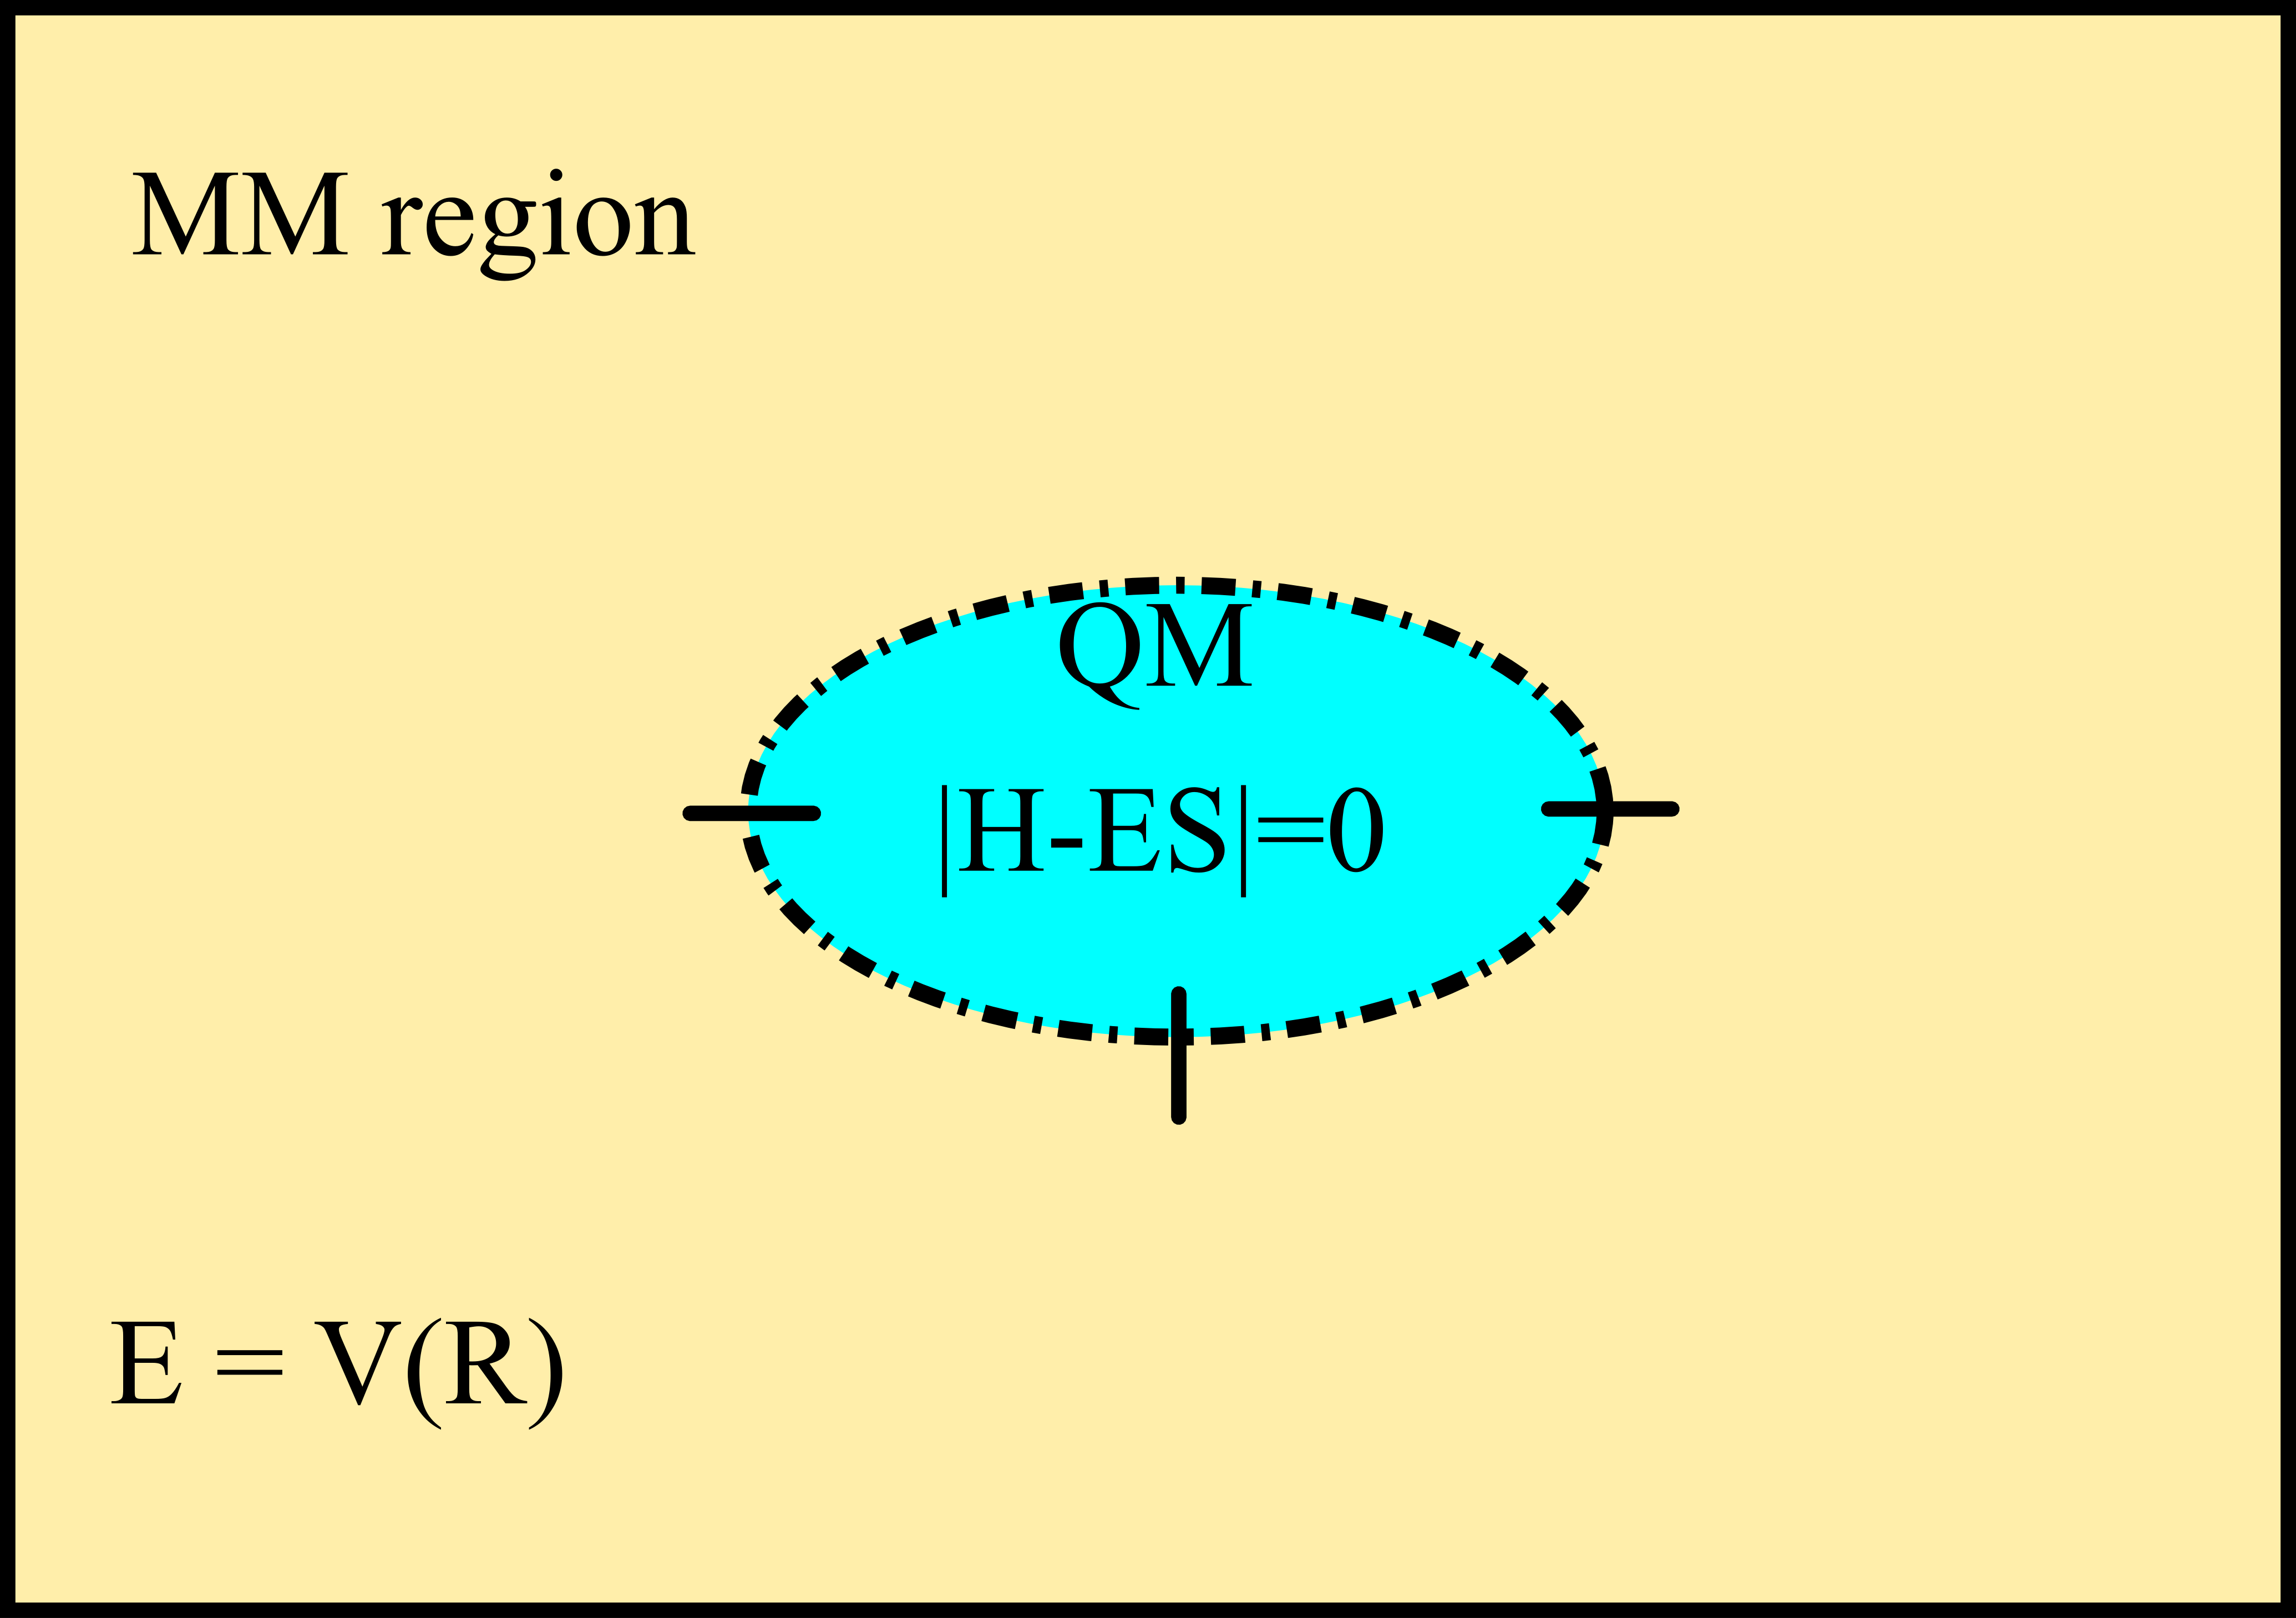
\includegraphics[scale=0.50]{../doc/images/QMMM_1.png}
 \caption{Schematic of a QMMM simulation box with bonds between the QM and MM
 regions.}
 \label{fig:QMMM1}
\end{figure}

QMMM calculations divide the system into regions which require accurate
quantum treatment and regions that can safely be approximated by classical
models (see Figure \ref{fig:QMMM1}).
The full effective Hamiltonian,
$\hat H_{eff}$, can be written as
\begin{equation}
 \hat H_{eff} = \hat H_{qm} + \hat V_{mm} + \hat V_{qmmm} \; ,
\end{equation}
where $\hat H_{qm}$ is the Hamiltonian for the QM region, $\hat V_{mm}$
is the classical potential for the MM region, and $\hat V_{qmmm}$ is the
potential for the interaction of the QM and MM regions. \\

Since the MM and QMMM interface are included only through the potential,
solving the Schr\"odinger equation is essentially trivial.
\begin{equation}
 E \approx \langle \psi |\hat H_{eff}|\psi \rangle
\end{equation}

\subsection{QM-MM interactions}

When the QM and MM regions are not connected by covalent bonds, the QM-MM
interactions are reasonably straightforward.
The interaction between the electric field of the MM region (point-charges or
multipoles) and the QM region is calculated by adding point-charges to the QM
calculations.
This allows for electrostatic repulsion and polarization, but neglects
exchange and dispersion interactions.
These missing interactions are added using the vdW potentials taken from the
MM force field. \\

For a single-point energy, the QM+charges calculation is performed with the QM
wrapper, while the MM wrapper calculates the MM energy with no charges or
bonded potentials on any of the QM atoms.
These two energies are then added together to get the total energy.
This approach splits $\hat V_{qmmm}$ between the MM calculation
($\hat V_{mm}$) and the QM calculation ($\hat H_{qm}$).

\subsection{Pseudo-bond method}

\begin{figure}[hbt]
 \centering
 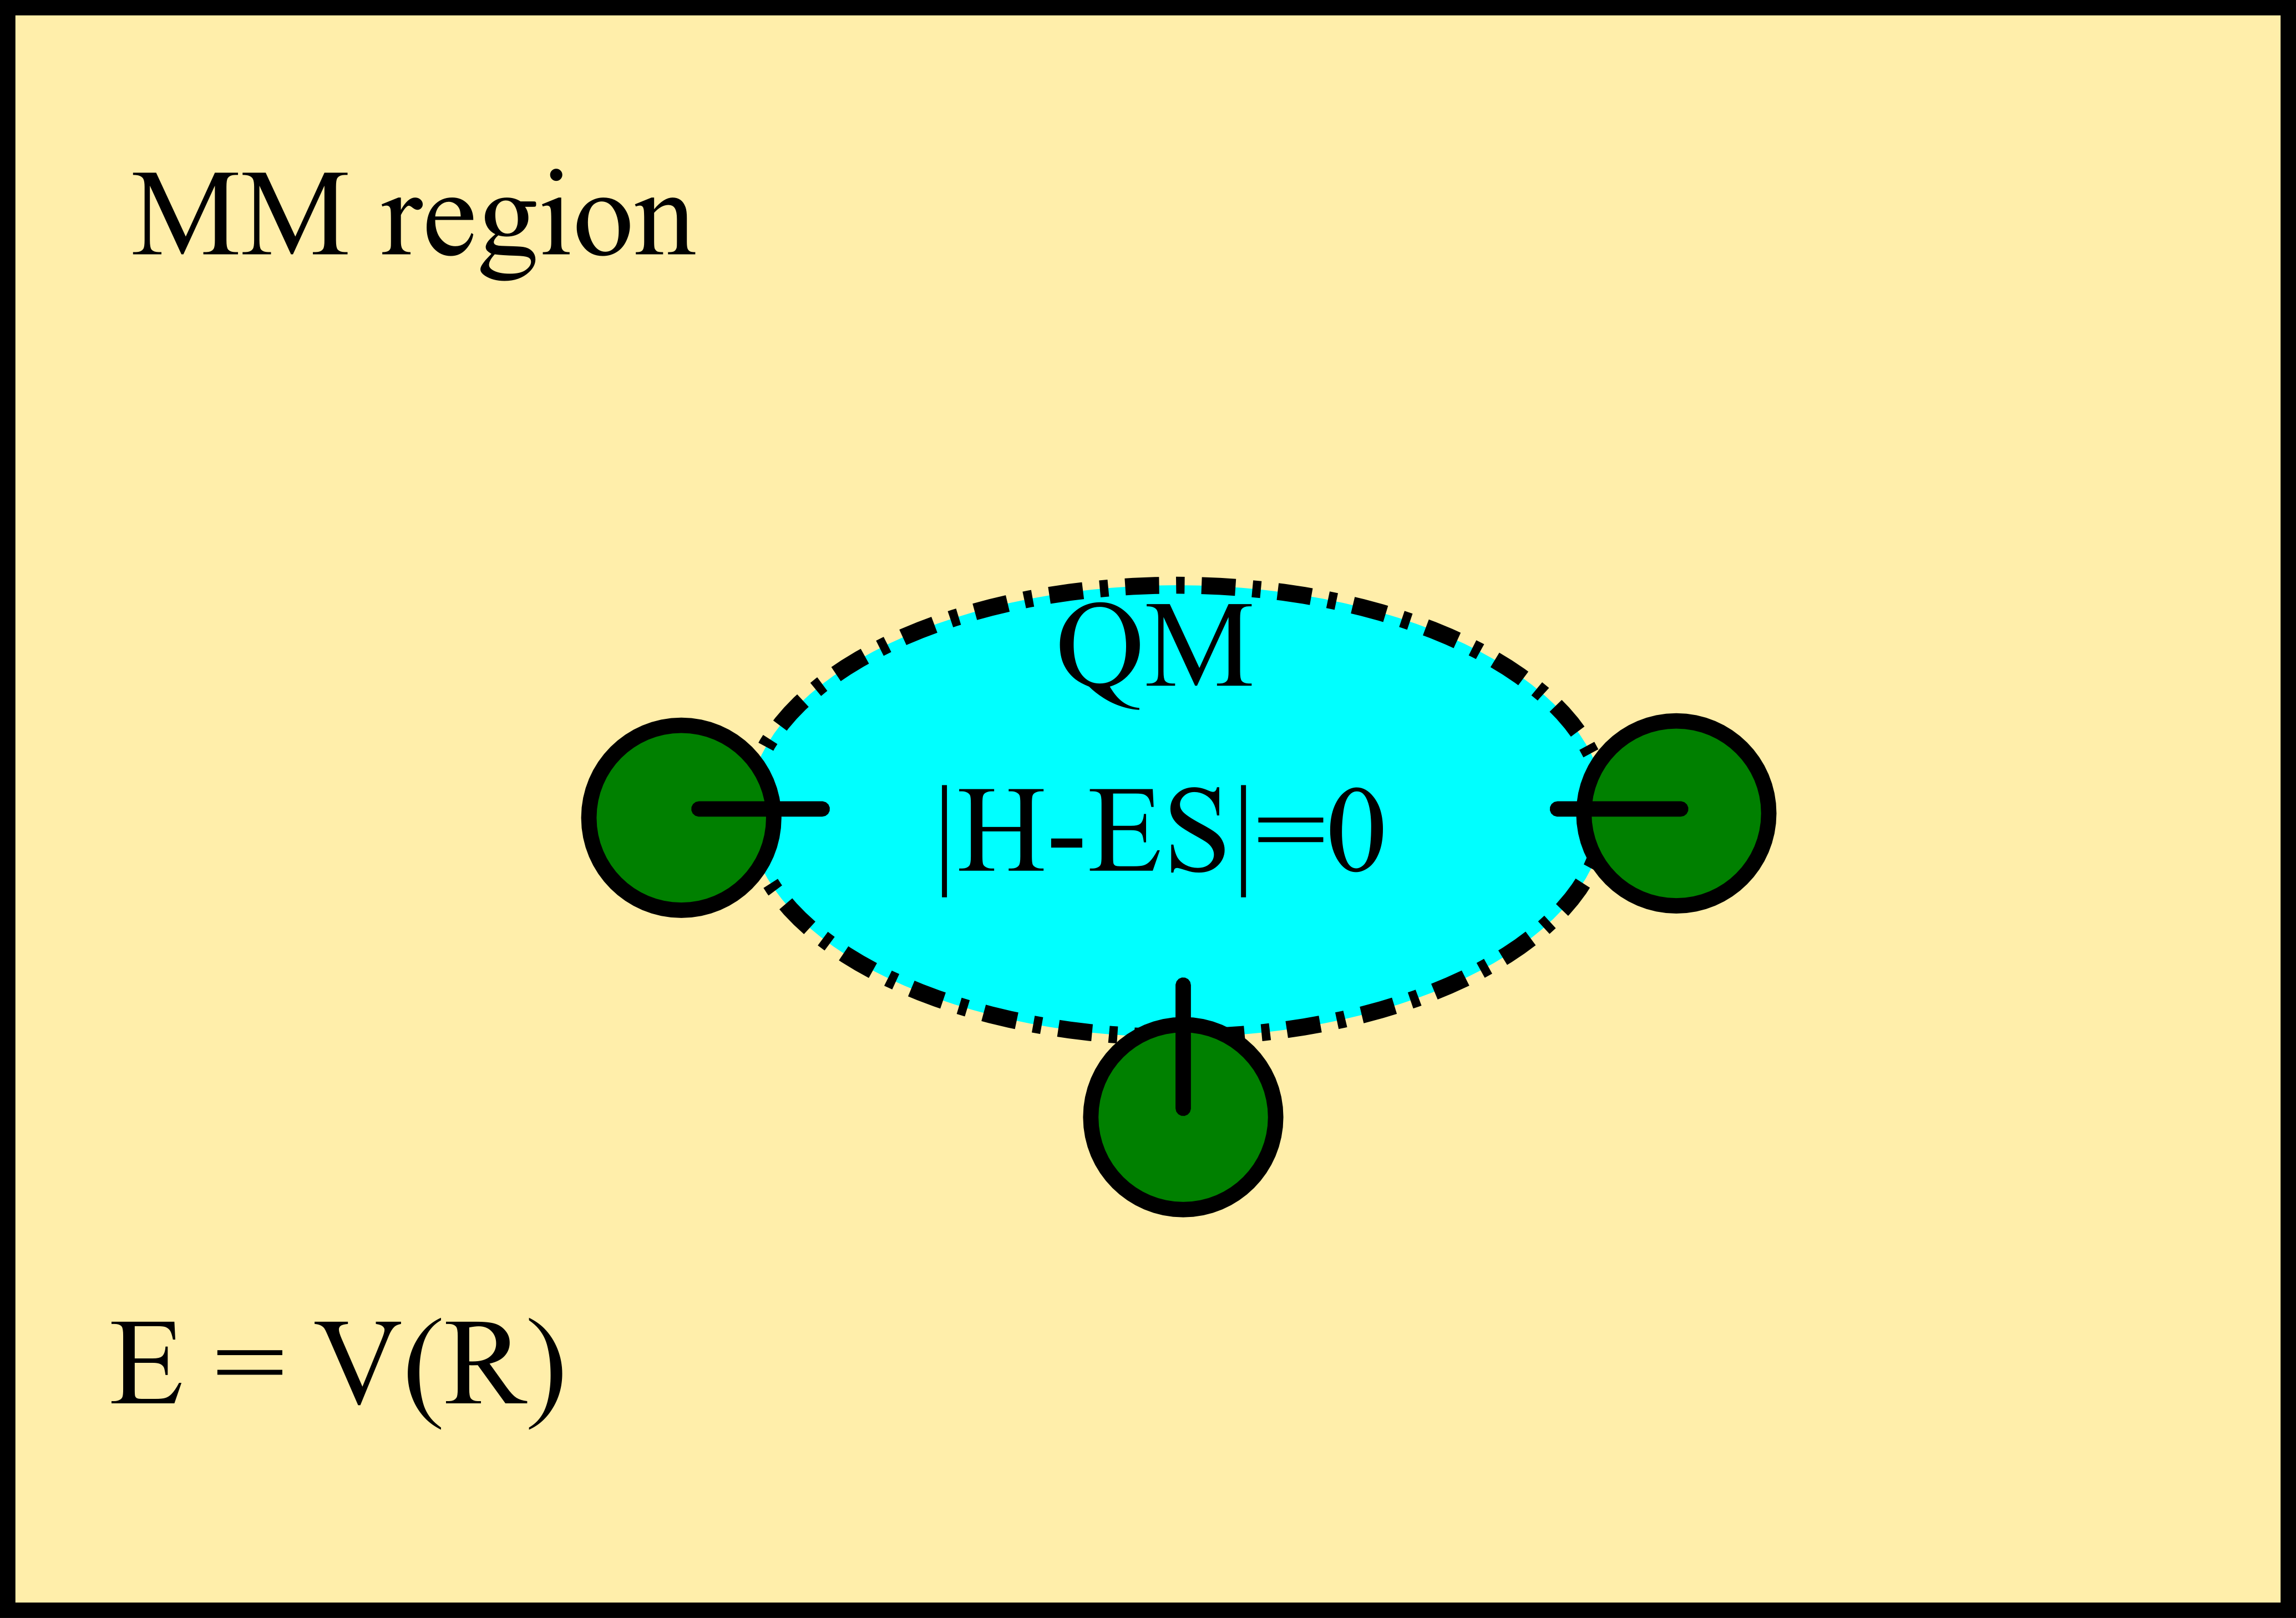
\includegraphics[scale=0.50]{../doc/images/QMMM_2.png}
 \caption{
 Schematic of a QMMM simulation box with the boundary region shown in
 green between the QM and MM regions.}
 \label{fig:QMMM2}
\end{figure}

\begin{table}[hbt]
 \centering
 \begin{tabular}{|c|c c|}
 \hline
  & \multicolumn{2}{|c|}{Wrapper calculation} \\
 Int.\ type & MM & QM \\ \hline
 MM-MM & FF & Zero \\
 QM-QM & Zero & $\rho_{el}$ \\
 PA-PA & FF & PP+$\rho_{el}$ \\
 BA-BA & FF & Zero \\
 QM-MM & FF-\{$q_{qm}$\} & $\rho_{el}$+\{$q_{mm}$\} \\
 QM-PA & Bonds & PP+$\rho_{el}$ \\
 QM-BA & FF-\{$q_{qm}$\} & Zero \\
 MM-PA & FF & PP+$\rho_{el}$+\{$q_{mm}$\} \\
 MM-BA & FF & Zero \\
 PA-BA & FF & Zero \\ \hline
 \end{tabular}
 \caption{
 The treatment of region-region interactions in the MM and QM
 wrappers during single-point energy calculations.
 Interactions were abbreviated as follows: force field (FF), electron density
 ($\rho_{el}$), pseudopotential (PP), no interaction (Zero), QM point-charges
 (\{$q_{qm}$\}), MM bond potentials (Bonds), and MM point-charges
 (\{$q_{mm}$\}).
 A "-" sign is used if the interaction is removed instead of added
 (i.e.\ FF-\{$q_{qm}$\} denotes the force field with no charges on the
 QM atoms).}
 \label{tab:IntTable}
\end{table}

\begin{figure}[hbt]
 \centering
 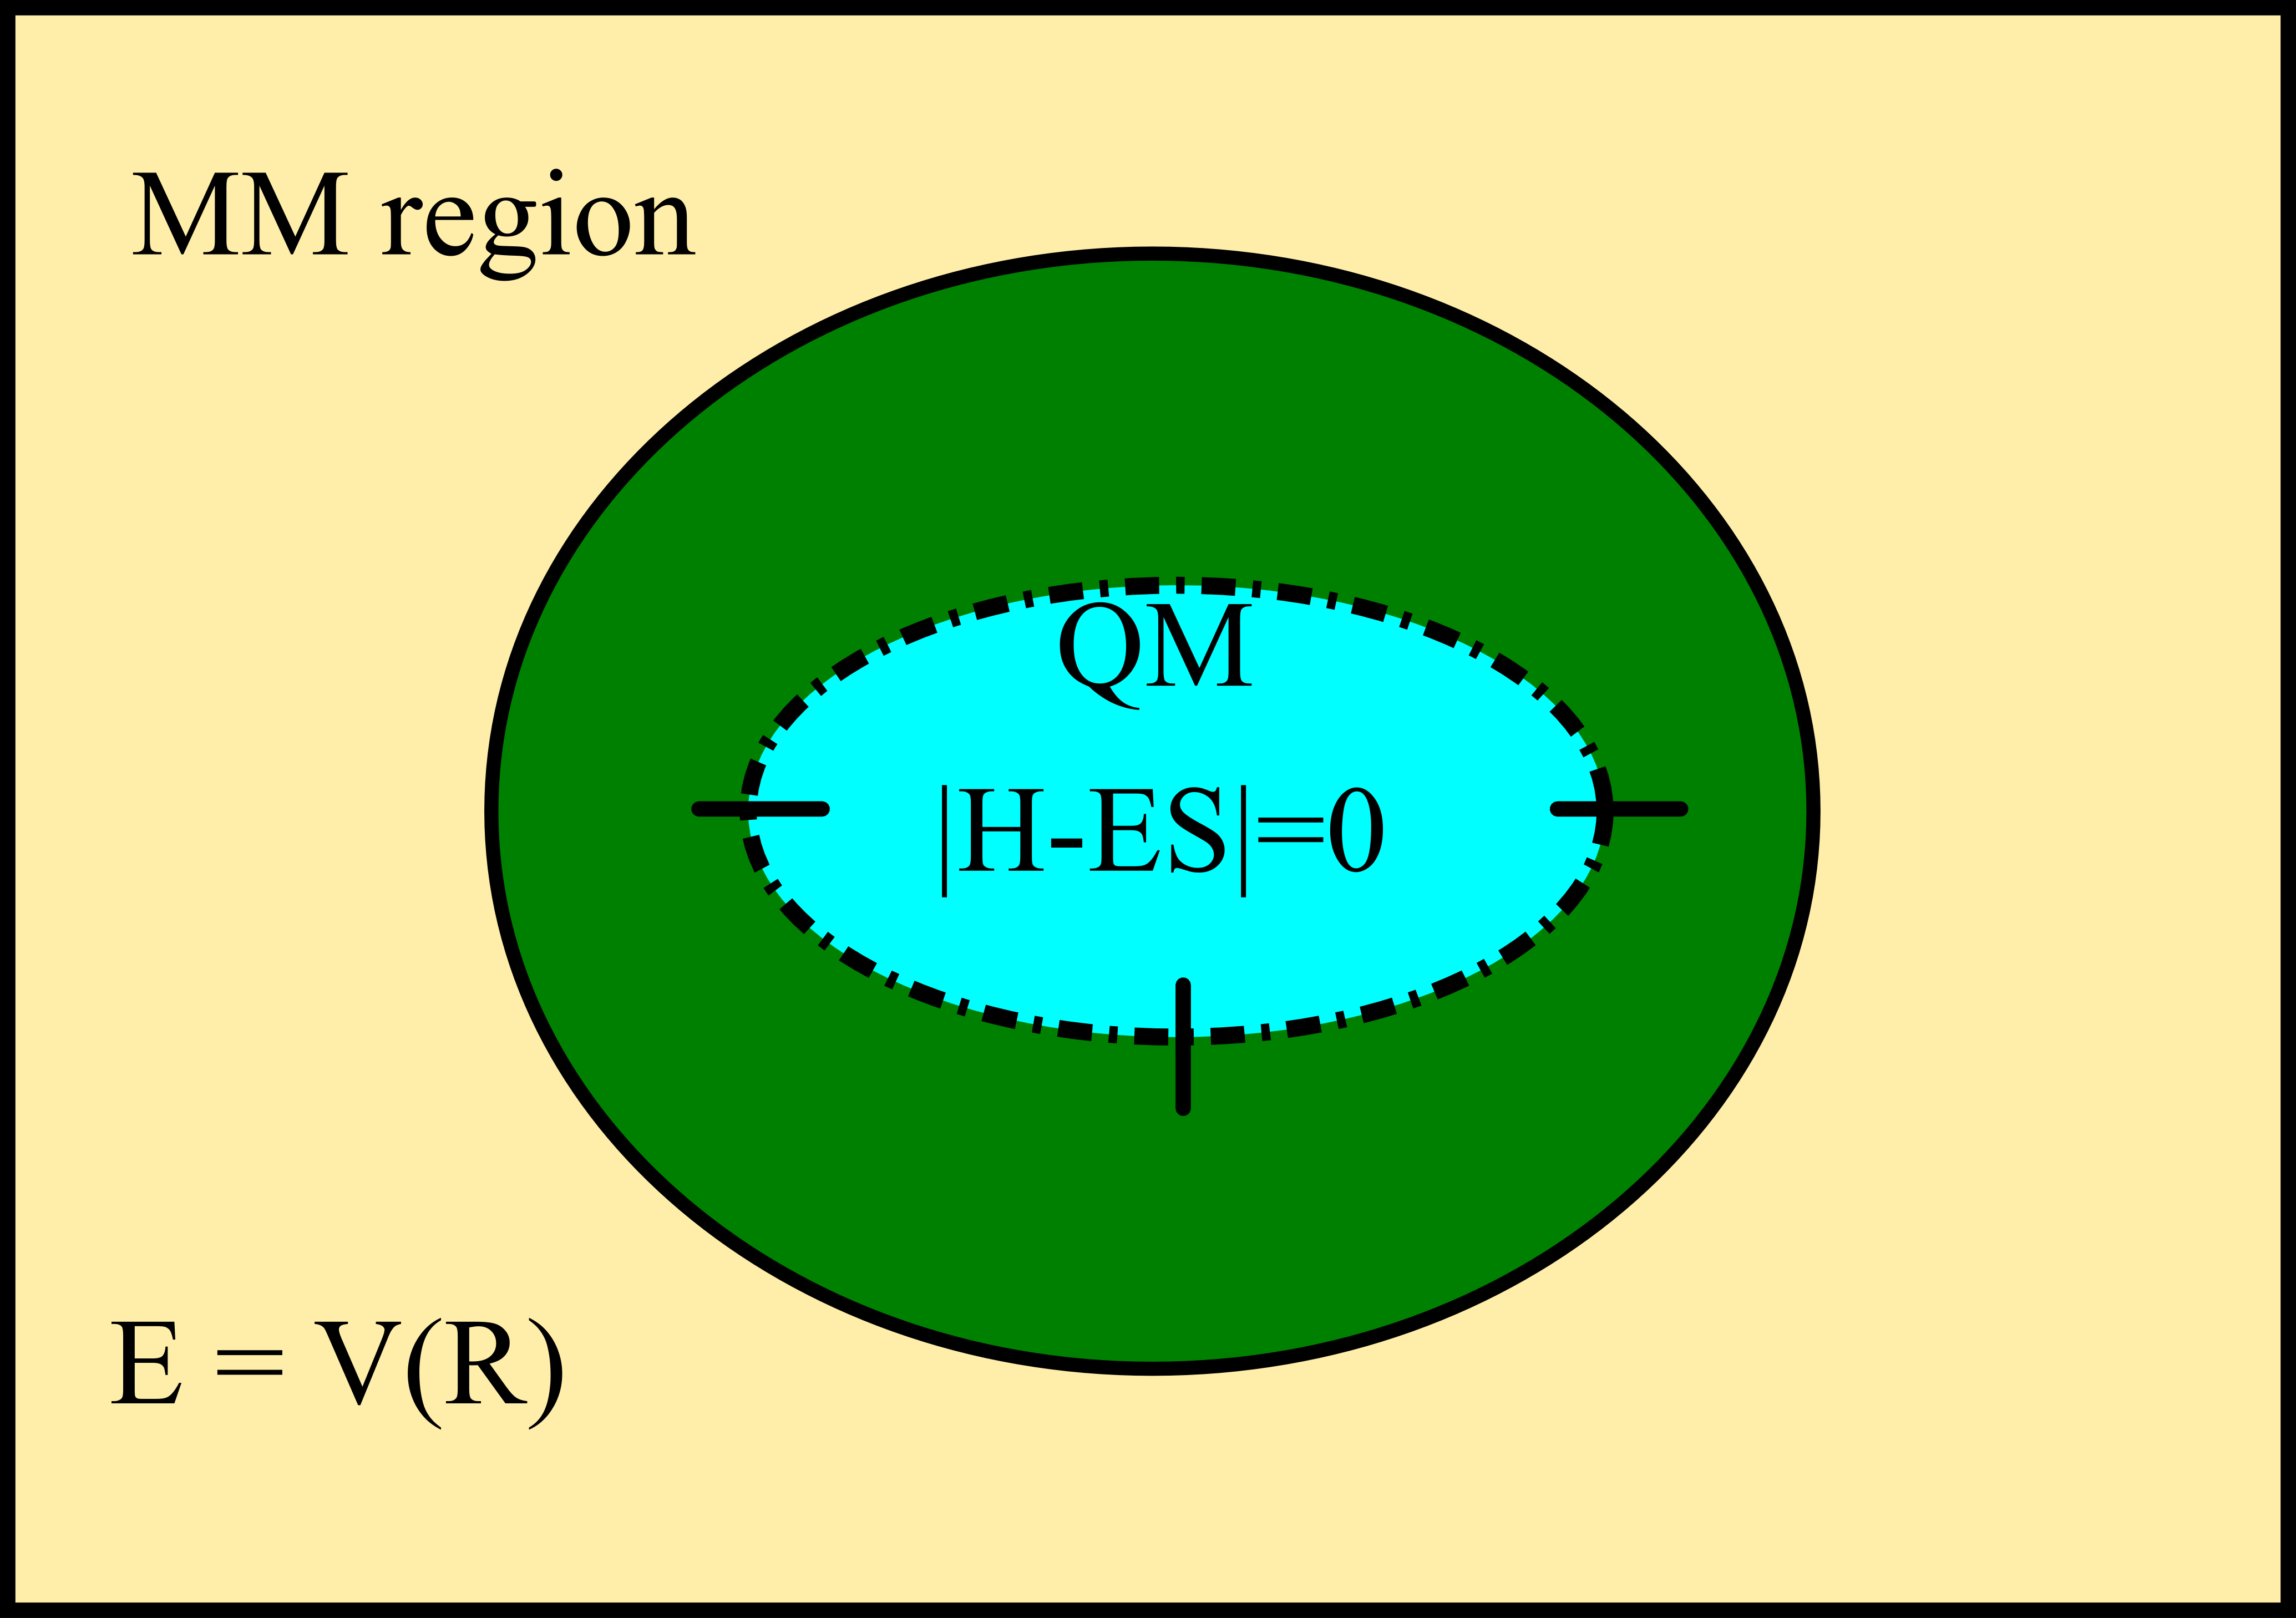
\includegraphics[scale=0.50]{../doc/images/QMMM_3.png}
 \caption{
 Schematic of a QMMM simulation box with a large boundary region
 between the QM and MM regions.}
 \label{fig:QMMM3}
\end{figure}

The calculations are more complicated when there are bonds between the QM and
MM regions.
Covalent bonds require two additional regions of the QMMM system,
a pseudo-bond (PB) region and a boundary atom (BA) region.
Pseudo-atoms are shared by the QM and MM regions, and handle the bulk of the
covalent interactions.
The severed bonds from the MM region are treated by adding a pseudopotential
to the pseudo-atoms that allows a fluorine atom to mimic the behavior of an
sp$^3$ hybridized carbon or nitrogen atom.
Boundary atoms correct for two additional errors.
First, having point-charges close to the QM region can cause the electron
density to be over-polarized.
The second error is introduced by the fact that the QM region must have an
integer number of electrons.
Both of these problems can be mitigated by absorbing the point-charges on the
atoms bonded to the pseudo-atoms into the QM region during the QM calculation.
This produces atoms with zero-charge on the boundaries between the QM and MM
regions. \\

For the MM part of the calculation, the pseudo-atoms and boundary atoms retain
their force field charges, and the MM bonding interactions are added for the
pseudo-atoms.
The treatment of different interaction types are given in Table
\ref{tab:IntTable} for single-point energy calculations.
In the pseudo-bond approach, only some of the bonded interactions are
calculated for the QMMM interface.
Further details on which bonded interactions are included can be found in the
literature. \\

So far we have discussed systems similar to the one shown in Figure
\ref{fig:QMMM2}, where the boundary atoms only surround the covalent bonds.
This is due to the primitive treatment of the QM-MM boundaries.
A more complicated scheme can be employed where the boundary atoms are
represented by a polarizable frozen density force field.
The QM and frozen density interactions are more natural than interactions
between the QM and point-charges, and thus, this approach avoids the
over-polarization.
Boundary atoms represented by frozen electron density can be extended further
from the QM region and can create smoother boundaries between the QM and MM
regions.
Ideally, a system could be constructed with a large boundary region between
the QM and MM regions (see Figure \ref{fig:QMMM3}).

\section{Monte Carlo Simulations}

\subsection{Stochastic sampling}

Monte Carlo simulations sample phase space by generation random changes to
the system.
Completely random sampling could eventually find a global minimum, however,
majority of the random structures would have energies well above $kT$ and
contribute very little to the statistical averages. \\

Almost any type of change can be made to the system in a Monte Carlo
simulation.
The primary limitations are the creativity of the programmer and the
efficiency of making the changes.
This allows Monte Carlo simulations to be tailored to the system and focus on
the randomly changing the most important features of a system. \\

If the moving atoms and/or type of random change are chosen randomly, this
procedure satisfies "detailed balance."
I.e.\ the move from configuration $i$ to configuration $j$ can be reversed by
a move from configuration $j$ to configuration $i$.

\subsection{Canonical ensemble}

A more efficient approach is to accept or reject the random moves based on
the Boltzmann weight of the configuration.
\begin{equation}
 P_{acc} \propto e^{-\Delta E\beta} \; ,
\end{equation}
where $P_{acc}$ is the probability of accepting the move, $\Delta E$ is the
change in energy, and $\beta$ is the inverse temperature,
\begin{equation}
 \beta = \frac{1}{kT} \; .
\end{equation}
This proceedure leads to biased sampling of the lower energy states. \\

Unlike molecular dynamics simulations, the natural ensemble for Monte Carlo
simulations is the canonical ensemble (NVT).
This is advantageous since there is no need to couple the simulation to a
thermostat.

\subsection{Isobaric-isothermal ensemble}

Although NVT simulations are natural for Monte Carlo, it is relatively easy to
change to the NPT ensemble.
NPT simulations are performed by randomly changing the volume of the
simulation box.
This procedure produces a slightly different expression for the probabilities,
\begin{equation}
 P_{acc} \propto e^{-(P\Delta V+\Delta E)\beta+N\Delta ln(V)} \; ,
\end{equation}
where $P$ is the pressure, $\Delta V$ is the change in volume, and $N$ is
the number of atoms.

\section{Path-Integral Monte Carlo}

\subsection{Path-integral formalism}

{\color{red}Comming soon...}

\subsection{PIMC simulations}

Path-integral Monte Carlo simulations are performed by simulating a large
number of classical systems which are then coupled together via harmonic
bonds.
Allowed Monte Carlo moves include random displacements of all beads in a
single atom, translations of an entire centroid, and volume changes. \\

The spring energy between the beads represents the quantum kinetic energy of
the centroid.
Moves are accepted based on the effective energy, $E_{eff}$
\begin{equation}
 E_{eff} = E_{spring}+\frac{1}{N_p}\sum_i^{N_p} E_{pot,i} \; ,
\end{equation}
where the spring energy is given by
\begin{equation}
 E_{spring} = \sum_{j}^{N_a} \frac{m_{j}N_{p}}{\hbar^2\beta^2}
              \sum_{i}^{N_p} (r_{i}-r_{i-1})^2  \; .
\end{equation}
Here the $N_a$ is the total number of atoms, $N_p$ is the number of beads,
$r_i$ is the position of bead $i$, and $E_{pot}$ is the potential energy.
The acceptance probability is given by
\begin{equation}
 P_{acc} \propto e^{\Delta E_{eff}\beta} \; .
\end{equation}

The path-integral total energy is slightly different from the effective
potential.
\begin{equation}
 \label{eq:PItotal}
 E_{pi} = \frac{3N_aN_p}{2\beta}-E_{spring}
          +\frac{1}{N_p}\sum_i^{N_p} E_{pot,i} \; ,
\end{equation}
where $E_{pi}$ is the total energy.
The first two terms in Eq.\ \ref{eq:PItotal} represent the classical kinetic
energy for all particles and the amount of kinetic energy absorbed by
centroid harmonic bonds.

\subsection{Ergodicity}

Classical Monte Carlo simulations typically scale as $N_a^2$ due to the
pairwise force field interactions of the atoms.
Since path-integral simulations have $N_p$ simulations that run in tandem,
the overall scaling is $N_pN_a^2$.
In addition to making the energy calculations computationally more expensive,
the efficiencies of the Monte Carlo moves tend to decrease.
Monte Carlo moves typically consist of changes to the positions of a single
atom or possibly more complicated moves where bond angles are shifted.
This leads to large systems changing very slowly and the path-integral
formalism essentially increases the size of the system. \\

Another problem introduced by the path-integral formalism comes from the
harmonic constraints between the beads.
The force constants for the path-integral springs is proportional to the mass
of the particle, which means that heavy atoms can experience very strong
forces holding the centroid close together.
The presence of strong potentials restricts the movement of the atoms, and
reduces $P_{acc}$.

\bibliographystyle{unsrt}
\bibliography{manual}

\end{document}
